\documentclass[a4paper,11pt,twoside,openright]{book}

\usepackage{latexsym}
\usepackage[latin1]{inputenc}
\usepackage[activeacute,spanish]{babel}
\frenchspacing
\usepackage{eucal}
\usepackage{multirow}
\usepackage{graphicx}
\usepackage[margin=1in,left=1.5in,includefoot]{geometry}
\usepackage{fancyhdr}
\usepackage{titling}
\usepackage{caption}
\usepackage{subcaption}
\usepackage{pgfplots}
\usepackage{amsmath}
\usepackage{fullname_esp}
\usepackage[colorlinks=true, linkcolor=blue]{hyperref}
\usepackage{pdfpages}
\usepackage{algorithmic}
\usepackage{algorithm}
\usepackage{listings}
\usepackage{color}
\usepackage{setspace}
\usepackage{mdframed}
%%%%%%%%%%%%%%%%%%%%%%%%%%%%%%%%%%%%%%%%%%%%%%%%%%%%%%%%
%%% SCRIPT DE TODO'S O TAREAS PENDIENTES CON BOCADILLOS.
%%%%%%%%%%%%%%%%%%%%%%%%%%%%%%%%%%%%%%%%%%%%%%%%%%%%%%%%
\usepackage{tikz}
\makeatletter \newcommand \listoftodos{\section*{Todo list} \@starttoc{tdo}}
\newcommand\l@todo[2]
    {\par\noindent \textit{#2}, \parbox{10cm}{#1}\par} \makeatother

\definecolor{orange}{rgb}{1,0.5,0}
\tikzstyle{notestyle} += [text width=\marginparwidth]
\tikzstyle{notestyleleft} += [text width=0.9\marginparwidth]
\tikzstyle{notestyle} = [draw=black, fill=orange, text width = 3cm]
\tikzstyle{notestyleleft} = [notestyle]
\tikzstyle{connectstyle} = [draw = orange, thick]
% Command for inserting a todo item
\newcommand{\todo}[1]{%
% Add to todo list
\addcontentsline{tdo}{todo}{\protect{#1}}%
%
\begin{tikzpicture}[remember picture, baseline=-0.75ex]%
    \node [coordinate] (inText) {};
\end{tikzpicture}%
%
% Make the margin par
\marginpar[%
{% Draw note in left margin
    \tikz[remember picture] \draw node[notestyleleft] (inNote) {#1};%
    \begin{tikzpicture}[remember picture, overlay]%
        \draw[connectstyle]
            ([yshift=-0.2cm] inText)
                -| ([xshift=0.2cm] inNote.east)
                -| (inNote.east);
    \end{tikzpicture}%
}%
]{% Draw note in right margin
    \tikz[remember picture] \draw node[notestyle] (inNote) {#1};%
    \begin{tikzpicture}[remember picture, overlay]%
        \draw[connectstyle]
            ([yshift=-0.2cm] inText)
                -| ([xshift=-0.2cm] inNote.west)
                -| (inNote.west);
    \end{tikzpicture}%
}%
}%

%%%%%%%%%%%%%%%%%%%%%%%%%%%%%%%%%%
%%%%%%%%%%%%%%%%%%%%%%%%%%%%%%%%%%

% MDFramed Config
\newcounter{passage}[chapter]\setcounter{passage}{0}
\renewcommand{\thepassage}{\arabic{chapter}.\arabic{passage}}
\newenvironment{passage}[2][]{
	\refstepcounter{passage}
	\ifstrempty{#1}
	{
		\mdfsetup {
			frametitle={
				\tikz[baseline=(current bounding box.east),outer sep=0pt]
				\node[anchor=east,rectangle,fill=blue!20] {
					\strut Passage~\thepassage
				};
			}
		}
	}
	{
		\mdfsetup {
			frametitle={
				\tikz[baseline=(current bounding box.east),outer sep=0pt]
				\node[anchor=east,rectangle,fill=blue!20] {
					\strut Passage~\thepassage:~#1
				};
			}
		}
	}
	\mdfsetup{
		innertopmargin=10pt,linecolor=blue!20,
		linewidth=2pt,topline=true,
		frametitleaboveskip=\dimexpr-\ht\strutbox\relax
	}
	\begin{mdframed}[]\relax%
	\label{#2}}{\end{mdframed}
}

%%%%%%%%%%%%%%%%%%%%%%%%%%%%%%%%%%
%%%%%%%%%%%%%%%%%%%%%%%%%%%%%%%%%%

\floatname{algorithm}{Algorithm}
\pagestyle{fancy}
\renewcommand{\chaptermark}[1]{\markboth{\textsc{Chapter} \thechapter. #1}{}}
\renewcommand{\sectionmark}[1]{\markright{\thesection\ #1}}

\fancyhf{}
\fancyhead[LE,RO]{\thepage}
\fancyhead[LO]{\rightmark}
\fancyhead[RE]{\leftmark}

%% Dejar espacio para la regla
\renewcommand{\headrulewidth}{0.02cm} %Son 0.5pt

% Redefinici�n de 'plain' para la primera p�gina del cap�tulo
\fancypagestyle{plain}{
\fancyhf{}
\renewcommand{\headrulewidth}{0pt}
\renewcommand{\footrulewidth}{0pt}
}

% Limpiar las cabeceras de las p�ginas que quedan completamente blancas
\makeatletter
  \def\cleardoublepage{\clearpage\if@twoside \ifodd\c@page\else
  \vspace*{\fill}
    \thispagestyle{empty}
    \newpage
    \if@twocolumn\hbox{}\newpage\fi\fi\fi}
\makeatother


\setlength\headheight{20pt}


%%%%%%%%%%%%%%%%%%%%%%%%%%%%%%%%%%%%%%%%%%%%%%
%%% COMIENZA EL DOCUMENTO
%%%%%%%%%%%%%%%%%%%%%%%%%%%%%%%%%%%%%%%%%%%%%%

\pagenumbering{roman}
\makeindex
\begin{document}

\newlength{\centeroffset}
\setlength{\centeroffset}{-0.5\oddsidemargin}
\addtolength{\centeroffset}{0.5\evensidemargin}
\thispagestyle{empty}
\vspace*{\stretch{1}}
\setstretch{1.2}

\noindent
\hspace*{\centeroffset}

\renewcommand\contentsname{Table of Contents}
\renewcommand\listfigurename{List of Figures}
\renewcommand\listtablename{List of Tables}
\renewcommand\bibname{References}
\renewcommand\figurename{Figure}
\renewcommand\tablename{Table} 
\renewcommand\chaptername{Chapter}
\renewcommand\appendixname{Appendix}
\renewcommand\abstractname{Abstract}



%%%%%%%%%%%%%%%%%%%%%%%%%%%%%%%%%%%%%%%%%%%%%%
%%% PORTADA
%%%%%%%%%%%%%%%%%%%%%%%%%%%%%%%%%%%%%%%%%%%%%%

\thispagestyle{empty}
\vspace*{1cm}
\hrule
\mbox{ }

\begin{center}
\begin{LARGE}
Final Master Project: Explainability of Language Models applied to Question Answering\\ [0.3em]
\end{LARGE}
\end{center}

\hrule
\vspace*{1cm}
\begin{center}
 
\includegraphics[width=0.3\textwidth]{images/Logo_UNED.jpg} %[width=4cm,,keepaspectratio]
\end{center}

\vfill
\begin{center}
  {\Large {\bf Final Master Project}}
\end{center}

\vfill
\begin{center}
  \textbf{Marcos Mart�nez Galindo} \\ [0.2em]
  Research project for the \\ \vspace{10pt}
  Master in Language Technologies\\ \vspace{10pt}
  National Distance Education University \\ \vspace{10pt}
  \vspace{2cm}
  Directed by \\ \vspace{10pt}
  \textbf{Prof. Dr. D. �lvaro Rodrigo Yuste} \\ [0.5em]
  June 2021\\
\end{center}


%%%%%%%%%%%%%%%%%%%%%%%%%%%%%%%%%%%%%%%%%%%%%%
%%% AGRADECIMIENTOS
%%%%%%%%%%%%%%%%%%%%%%%%%%%%%%%%%%%%%%%%%%%%%%
%\chapter*{Agradecimientos}
%\label{sec:Agradecimientos}

%\noindent Agradecimientos si procede.


%%%%%%%%%%%%%%%%%%%%%%%%%%%%%%%%%%%%%%%%%%%%%%
%%% RESUMEN
%%%%%%%%%%%%%%%%%%%%%%%%%%%%%%%%%%%%%%%%%%%%%%
%\chapter*{Resumen}
%\label{sec:Resumen}
%\noindent Breve resumen del trabajo realizado y de los objetivos conseguidos.


%%%%%%%%%%%%%%%%%%%%%%%%%%%%%%%%%%%%%%%%%%%%%%
%%% ABSTRACT
%%%%%%%%%%%%%%%%%%%%%%%%%%%%%%%%%%%%%%%%%%%%%%
\chapter*{Abstract}
\label{sec:Abstract}
\noindent Breve resumen del trabajo realizado y de los objetivos conseguidos en ingl�s.


%%%%%%%%%%%%%%%%%%%%%%%%%%%%%%%%%%%%%%%%%%%%%%
%%% INDICES
%%%%%%%%%%%%%%%%%%%%%%%%%%%%%%%%%%%%%%%%%%%%%%
\tableofcontents
\listoffigures
\listoftables


%%%%%%%%%%%%%%%%%%%%%%%%%%%%%%%%%%%%%%%%%%%%%%
%%% ENTRADAS A LOS FICHEROS CON LOS CAPITULOS
%%%%%%%%%%%%%%%%%%%%%%%%%%%%%%%%%%%%%%%%%%%%%%
%%%%%%%%%%%%%%%%%%%%%%%%%%%%%%%%%%%%%%%%%%%%%%
%%% INTRODUCCION
%%%%%%%%%%%%%%%%%%%%%%%%%%%%%%%%%%%%%%%%%%%%%%

\chapter{Introduction}
\fancyhead[RE]{\textsc{Chapter} \thechapter. Introduction}
\label{ch:Introduction}
\pagenumbering{arabic}

\section{Motivation}
\label{sec:Motivation}
\noindent

\section{Proposal and goals}
\label{sec:ProposalAndGoals}
\noindent

\section{Document structure}
\label{sec:DocumentStructure}
\noindent

\begin{description}
\item \textbf{Chapter 1. Introduction.} In this chapter the main motives for the realization of this essay, the proposal and the goals to achieve are presented, as well as the document structure.
\item \textbf{Chapter 2. State of the art.} The discipline and the task are reviewed in this chapter, including a brief introduction of the explainability, the language models and the question answering task and the state of the art of this areas. At the end of this chapter, the state of the art of explainability applied to Natural Language Processing tasks is reviewed.
\item \textbf{Chapter 3. Methodology.}  The different methods and algorithms used to solve the problem are introduced and studied in this chapter.
\item \textbf{Chapter 4. Results.} After knowing the different methods and algorithms being used, the experiments with their results are presented in this chapter.
\item \textbf{Chapter 5. Conclusions and future work.} The conclusions of the review of the state of the art in addition to the conclusion of the usage of the different methods and to the future work that could be done after this project.
\end{description} 
%%%%%%%%%%%%%%%%%%%%%%%%%%%%%%%%%%%%%%%%%%%%%%%%%%%
%%% ESTADO DEL ARTE
%%%%%%%%%%%%%%%%%%%%%%%%%%%%%%%%%%%%%%%%%%%%%%%%%%%

\chapter{State of the Art}
\fancyhead[RE]{\textsc{Chapter} \thechapter. State of the art}
\label{ch:StateOfTheArt}
\noindent

\section{Language models}
\label{sec:LanguageModels}
\noindent In 2001, Joshua Bengio et al. proposed the first neural language model, based on a feed-forward neural network.\cite{Bengio2001} However, it wasn't until 2013 that neural networks begin to gain relevance in the world of \emph{NLP}, and it was due to the \emph{word embeddings} and the new neural architectures, like \emph{Recurrent Neural Networks} (\emph{RNN}).
\paragraph{}
The \emph{word embeddings} are vectorized representantions of the words contained in a document, and since its begining have gained a lot of importance in the world of the \emph{NLP}, because they are able to capture the context of the word within the text, improving the way the model understands the text. This way, a polysemic word has not the same representation in different contexts. One example of this techinque is \emph{Word2Vec}, probably the most used technique by the researchers to learn the \emph{word embeddings} of the text, and was developed by Tomas Mikolov in 2013.\cite{Mikolov2013}.
\begin{figure}[h!]
	\centering
	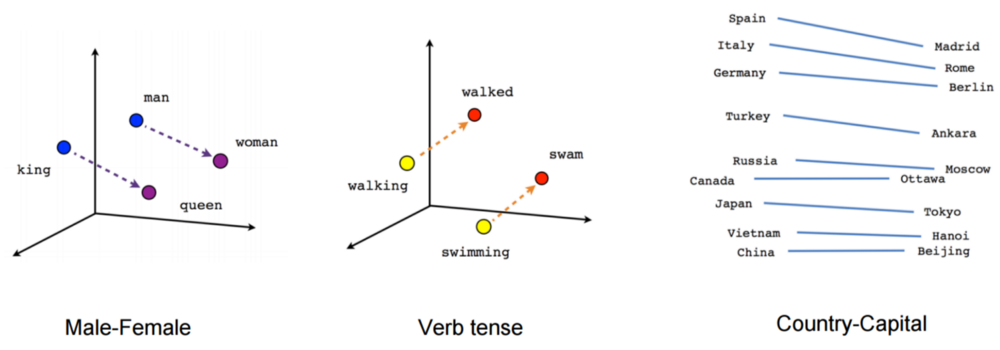
\includegraphics[scale=0.35]{images/wordembeddings}
	\caption{Word Embeddings}
	\label{fig:wordembdedding}
\end{figure}
\paragraph{}
When dealing with temporal series or data sequences, neural networks are not able to model the temporal dependency, as they don't have knowledge about the previous sequences. To solve this, a new variety of neural networks was developed, the \emph{RNN}, that have the ability to process data sequences by saving memory of the already processed ones. In \emph{NLP} this is really important, because in natural language texts a single word is not enough to capture its meaning, also the previous words (or sentences) are needed, so the ability to save ``memory'' about the previous words improved the performance of neural networks in almost every \emph{NLP} task. Thus, a lot of versions of neural netowrks have been developed, like the \emph{Long Short-Term Memories} (\emph{LSTM}), that are very used in \emph{NLP} because they save the memory during more time than other versions, increasing the window size of the sequences being seen.
\begin{figure}[!h]
	\centering
	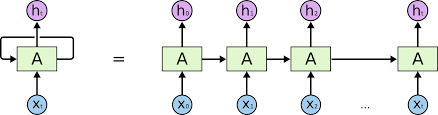
\includegraphics[scale=0.55]{images/lstm}
	\caption{\emph{LSTM} Recurrent Neural Networks.}
	\label{fig:lstm}
\end{figure}
\paragraph{}
Other architecture that has revolutionized the research world in \emph{NLP}, contributing to the appearance of new language models is the \emph{encoder-decoder} architecture, based on two different parts, the \emph{encoder} that codifies the input, getting a vectorized representation that is transmitted to the sencond part, the \emph{decoder}, that from this codified sate generates the output. Usually, a sentence is given as input and the output is a new sentence, so that this architecture is also known as \emph{sequence to sequence}. In its begining it was used to \emph{machine translation} task, having as input a text in some language and the translation as output.
\begin{figure}[h!]
	\centering
	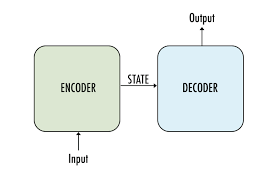
\includegraphics[scale=0.75]{images/encoderdecoder}
	\caption{\emph{Encoder-Decoder} architecture.}
	\label{fig:encoderdecoder}
\end{figure}
\paragraph{}
One of the main problems of this architecture is the need of codify the whole input before the output generation, that is done by looking at the whole input. The \emph{attention} mechanism was developed to solve this, giving as input for the \emph{decoder} not only the codified state of the input (as in the classic \emph{encoder-decoder} architecture) but also the hidden states of the \emph{encoder}, that now process the input splitted, making possible to look only at one part of the input and not the whole input as before.\cite{Bahdanau2014} 
\begin{figure}[h!]
	\centering
	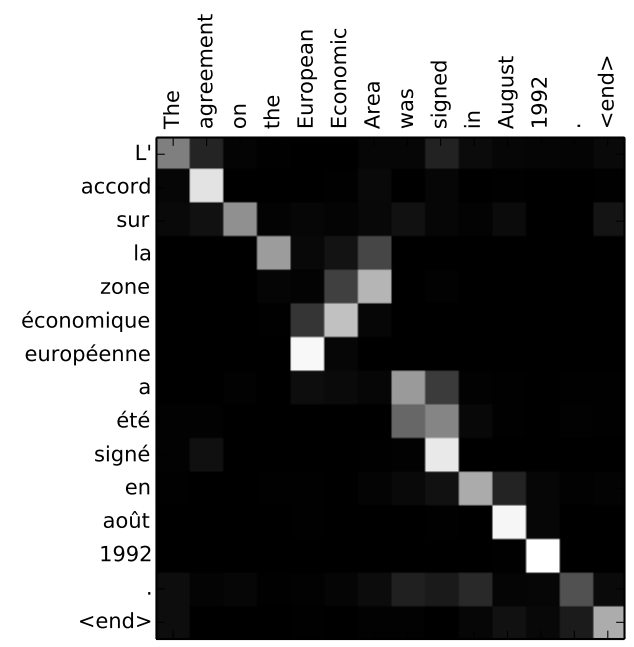
\includegraphics[scale=0.35]{images/attention}
	\caption{Example of the \emph{Attention} mechanism in machine translation. It can be seen as the \emph{Attention} mechanism focus only on the words being translated and the relevant ones instead in the whole sentence.}
	\label{fig:attention}
\end{figure}
\paragraph{}
Three years later, in 2017, probably the most important article in the history of \emph{NLP} was released: ``Attention is all you need''.\cite{Vaswani2017} In the article, Vaswani et al. propose a novel neural architecture based only on layers using the \emph{Attention} mechanism, the \emph{Transformer}. Besides, the \emph{Transformers} use a variation of the \emph{Attention} mechanism called \emph{Self-Attention}, that allows to take as input other positions of the self input, which makes possible to use other words of the same input to codify each word, as can be seen in Figure \ref{fig:selfattention}.
\begin{figure}[h!]
	\centering
	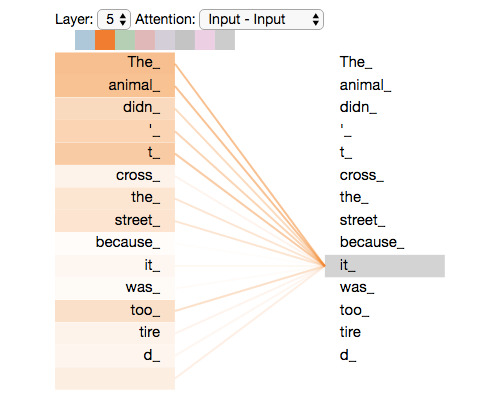
\includegraphics[scale=0.45]{images/selfattention}
	\caption{\emph{Self-Attention} mechanism.}
	\label{fig:selfattention}
\end{figure}
\paragraph{}
In the \emph{Transformer}, the output of different \emph{Self-Attention} layers are concatenated, creating a muli-dimensional \emph{Attention} representation, what is the \emph{Multi-Head Attention}. This way, each head can learn to codify the same word in different ways, what allows the model to capture more information of the word. Although it can be considered as \emph{Transformer} every architecture designed to process a set of words with the \emph{Attention} mechanism as the unique way of interaction between them, the basic structure of the \emph{Transformer} is based on:
\begin{itemize}
\item \emph{Self-Attention} or \emph{Multihead Attention} layer.
\item Normalization layer.
\item \emph{Feed-forward} layer.
\item Normalization layer.
\item Residual connections.
\end{itemize}
With this, an \emph{encoder-decoder} architecture is developed, as shown in Figure \ref{fig:transformer}.
\begin{figure}[h!]
	\centering
	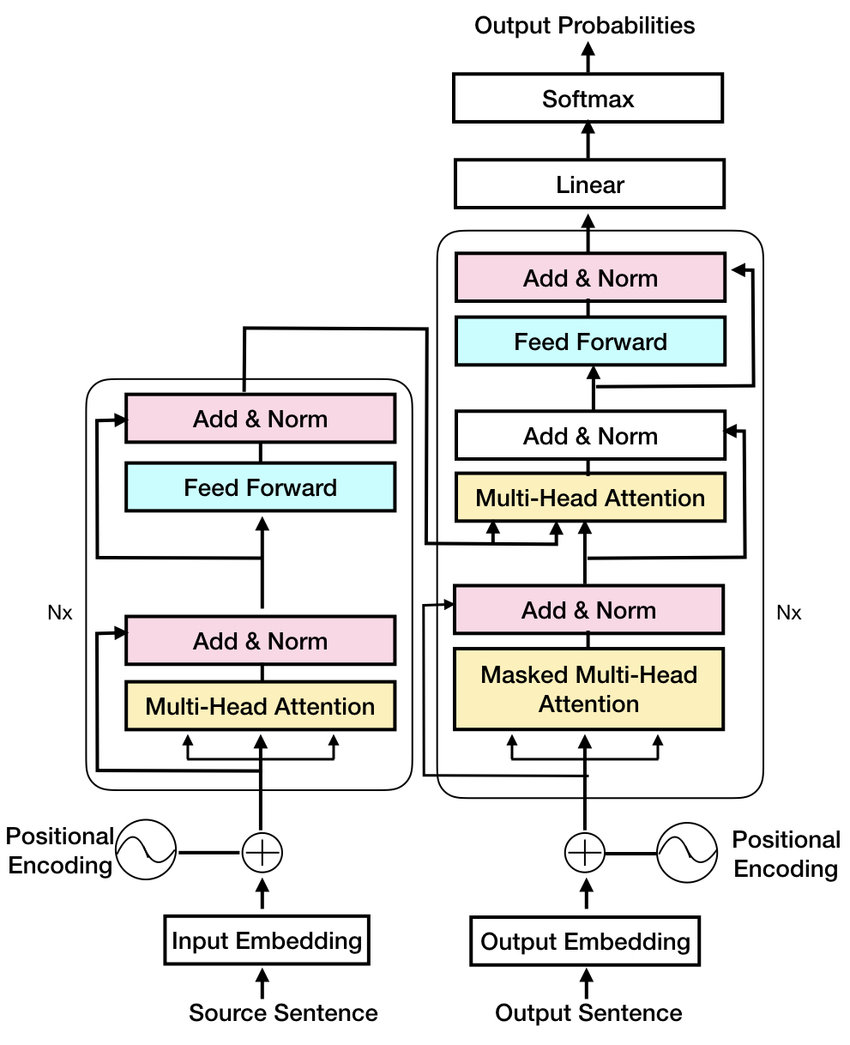
\includegraphics[scale=0.25]{images/transformer}
	\caption{\emph{Transformer} architecture.}
	\label{fig:transformer}
\end{figure}
\paragraph{}
Another one of the key points to the massive expansion of the language models has been the training techniques used. Along the history of the language models, they used to be unidirectionals, this is, to predict the next word they used only the words before. But this changed with the arrival of \emph{BERT}, \emph{Pre\-training of Deep Bidirectional Transformers for Language Understanding}. \cite{Devlin2018} Instead of predict the next word, \emph{BERT} masks randomly some tokens in the input, and trains by trying to predict the original words that have been masked, using both left and right sides of the sentences (bidirectional), which allows the model to capture more information while codifying the tokens. This is known as \emph{Masked Language Models}, \emph{MLM}.
\paragraph{}
Although the most common way to work is dealing with words, the language models can work in different ways, like for example using \emph{n-grams} and using smooth techniques to deal with \emph{n-grams} neer seen before\cite{Knesser1995}. Another ones, like \emph{ProphetNet} \cite{Yan2020}, try to predict not only the next token, but the $n$ following tokens.
\paragraph{}
So, the basic idea behind the language models is to predict the next token, but they can be used also for other \emph{NLP} tasks such as \emph{Question Answering}. To achieve this, different aditional layers are set on top of the language model, trained to solve the specific task, taking as input the output of the language model, this is, the original input tokenized. 
\paragraph{}
Therefore, there are two different parts, the language model and the specific layers, and there are also two different types of trainings, the one used to train the language model (without the specific layers), that can be trained using massive amounts of texts, like the \emph{Wikipedia}, and the one used to train the model to the specific task, which requires a specific \emph{dataset}, which is known as \emph{fine-tuning}.
\subsection{Main Language Models for Question Answering}
\noindent Since the release of \emph{BERT} the number of papers and models published has suffered an exponential grown, Figure \ref{fig:cronology}, most of them using the same architecture than \emph{BERT}, or with little variations.
\begin{figure}[h!]
	\centering
	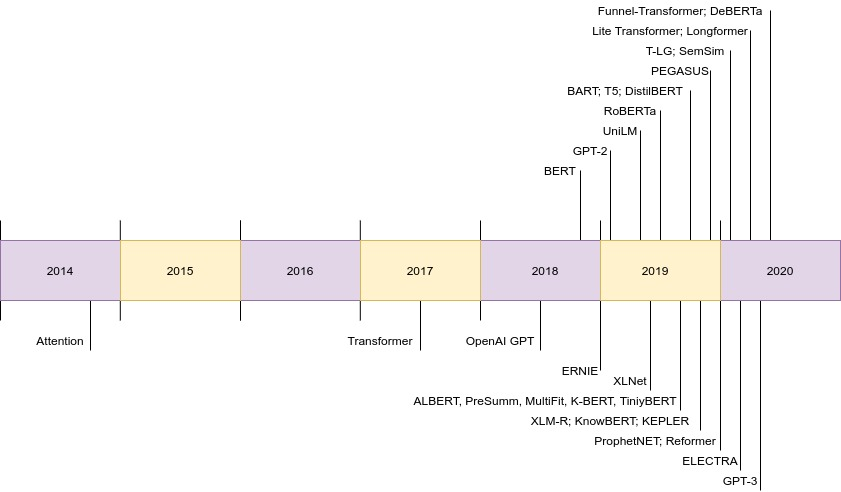
\includegraphics[scale=0.35]{images/cronology}
	\caption{Cronological view of a sample of language models. It can be seen that since \emph{BERT} the number of language models released has grown exponentially.}
	\label{fig:cronology}
\end{figure}
So, after a research of the state of the art of language models, it has been developed a brief review of some of the most interesting models.
\subsubsection{BERT}
\noindent As said before, the ``boom'' of the \emph{LM} started with \emph{BERT}, \emph{Pre\-training of Deep Bidirectional Transformers for Language Understanding}\cite{Devlin2018}. In this article, Devlin et al. propose a novel architecture based on the classic \emph{encoder-decoder} but, in this case, made only with \emph{Transformers}. There were released two different versions of \emph{BERT} depending on its size: one with 12 layers and 110 million parameters (the same as the \emph{OpenAI GPT} for comparison purposes); and one with 24 layers and a total number of 340 million parameters.
\paragraph{}
The \emph{WordPiece} embeddings (\cite{Wu2016}) are used, with a total umber of 30.000 \emph{tokens} in the vocabulary. The first \emph{token} of each sequence (understanding as sequence not a sentence of the text, but the input given to \emph{BERT} than can be up to two sentences) is a \emph{{CLS} token}, sentences in the input sequence are separated by a \emph{[SEP] token}.
\paragraph{}
In addition to this, a (not) new training is used, in which some random \emph{tokens} are masked (replaced by a \emph{[MASK] token}), and the model has to predict which one was the original \emph{token}. Altough this method started to be famous thanks to \emph{BERT} it wasn't invented by Devlin et al., but it was known as \emph{Cloze} task in the literature \cite{Taylor1953}. In the article, the authors explain that while training \emph{BERT} a 15\% of the \emph{tokens} is `masked''. When masking a \emph{token}, there are 3 possibilites:
\begin{enumerate}
\item The \emph{token} is replaced by a \emph{[MASK] token} 80\% of the time.
\item The \emph{token} is replaced by a random \emph{token} 10\% of the time.
\item The \emph{token} is not changed 10\% of the time.
\end{enumerate}
But this is not the only way \emph{BERT} is trained. It is also trained for another task, the prediction of the next sentence, \emph{NSP} (Next Sentence Prediction). In this task, two sentences are selected from the text ($A$ and $B$). 50\% of the time $B$ is the sentence that really follows $A$, meanwhile a 50\% of the time is not. In this task $BERT$ has to classify if $B$ is the next sentence following $A$ or not. 
\subsubsection{T5}
\noindent \emph{T5}, created by Raffel et al. in Google, in 2019.\cite{Raffel2019} is a model proposed in an extense research article with mulitple tests of diferent architectures based on \emph{Transformers} and with a mask training, the same used by \emph{BERT}.
\paragraph{}
Besides the high-quality research presented, \emph{T5} does not propose any novel architecture, but due to its high size and its training over a really big \emph{corpus} obtained from the \emph{World Wide Web} (known as \emph{C4}, \emph{Colossal Clean Crawled Corpus}), \emph{T5} obtains state-of-the-art performance in multiple \emph{NLP} tasks, such as \emph{Question Answering}.
\subsubsection{GPT-2/GPT-3}
\emph{GPT} architectures, \cite{Openai}\cite{Radford2019}\cite{Brown2020}, are a group of language models based on an architecture based only on \emph{decoders}, without the encoder that is habitual in language models. These decoders layers are trained predicting next words, without a masked training, as it used to be in the past, which is known as ``from left to right''. This way, the model can only see the words at the left of the token being processed, loosing some of the context, but the quality of the generated text in \emph{Natural Language Generation} (\emph{NLG}) tasks is usually of a higher quality, because in runtime while generating new text, the model can only see the text at the left of the word.
\begin{figure}[h!]
	\centering
	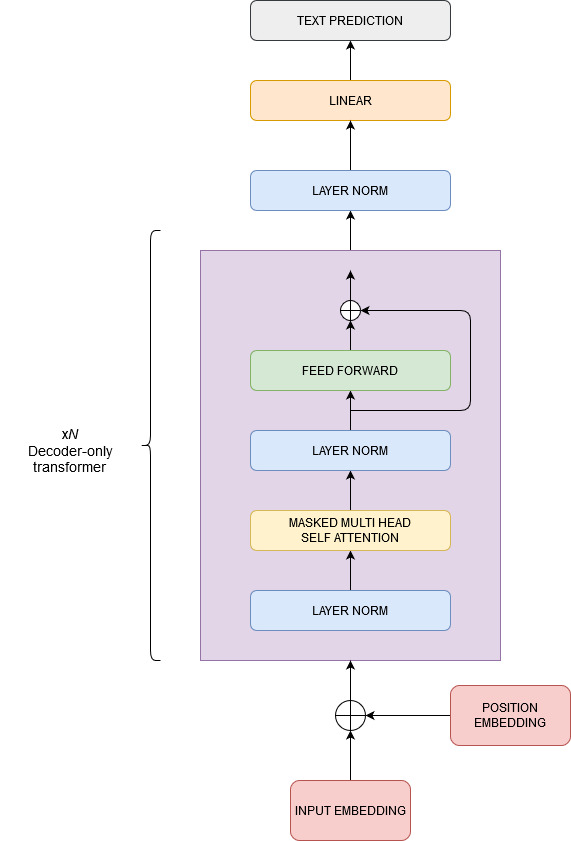
\includegraphics[scale=0.45]{images/gpt2}
	\caption{\emph{GPT-2} architecture.}
	\label{fig:gpt2}
\end{figure}
\paragraph{}
\emph{GPT-2} architecture caused quite a stir among all the researchers in \emph{NLP} (and also in the news), due to the quality of its generated text. But it also demonstrated that \emph{LM} are able to generalize and solve tasks without a specific \emph{fine-tuning} for the task. This way, \emph{GPT-2} was trained on a huge \emph{corpus}, but it was not trained for a specific training such as \emph{QA}. Even when the results are not as good in the benchmarks as the ones obtained from other models trained specifically for the task, results are really good, especially in \emph{NLG} tasks, which is surpisingly due to the fact that the model has not been trained for that.
\paragraph{}
The \emph{dataset} used to train \emph{GPT-2} is known as \emph{WebText}, and was generated from posts of the social network \emph{Redit}. To assure a good quality of these posts, only those who had a high punctuation were used, obtaining this way a set of texts well-written and covering different topics.
\paragraph{}
But, again, it wasn't trained for a specific tasks. Nevertheless, posts in \emph{Redit} are written by real people interacting with each other, so the model has been able to learn how to solve different tasks of \emph{NLP}. For example, in these posts some users made a question that other users answered, and this way the model learned to answer questios. 
\paragraph{}
Other interesting example is for the \emph{Text Summarization} (\emph{TS}) task, which consists on generate an abstract from a text. In these posts, users used to add a brief summary at the end of the post, tagged with the acronym \emph{TL;DR:} (Too Large; Didn't Read:). Researchers found that if this token is added to the model at the end of the input, the text generated by \emph{GPT-2} is the summary of the input, solving the \emph{TS} task.
\paragraph{}
When \emph{GPT-2} was released its large size was surprised (1.542 millions - 48 \emph{decoder} layers), which makes possible to understad the text and to generate a high quality output. But now the size of \emph{GPT-2} is not even close to the largest models used in \emph{NLP}.
\paragraph{}
Its ``big brother'', \emph{GPT-3}, its the largest model by the date of this article, with 175.000 millions of parameters, what allows it to understand the language in a way never seen before. Its able to solve any task in any domain without needing to adapt it with a specific \emph{fine-tunnning}, which is known as \emph{zero-shot}.
\paragraph{}
Its also able to solve, not only \emph{NLP} tasks, but also even arithmetic operations up to 3 digits, something really impressive that demonstrates its knowledge beyond the languages.
\subsubsection{Turing NLG}
\noindent \emph{Turing NLG} or \emph{T-NLG}\cite{Rosset2020} its a model developed by \emph{Microsoft} and, till the release of \emph{GPT-3} was the largest model published, with 17.000 millions of parameters (10 times less than \emph{GPT-3}). Nevertheless, its still a really massive amount of parameters, wich allows \emph{T-NLG} to reach state-of-the-art performance in almost any \emph{NLP} task, such \emph{QA} or \emph{TS}.
\paragraph{}
Due to it large size, the \emph{Microsoft} team developed a \emph{Deep Learning} library (\emph{DeepSpeed}) and a new optimizer (\emph{ZeRo}) that allow the parallelization in the optimiziation and reduce the resources needed by the model to make possible the training of large models in a more efficient way, with less resources.
\begin{figure}[h!]
	\centering
	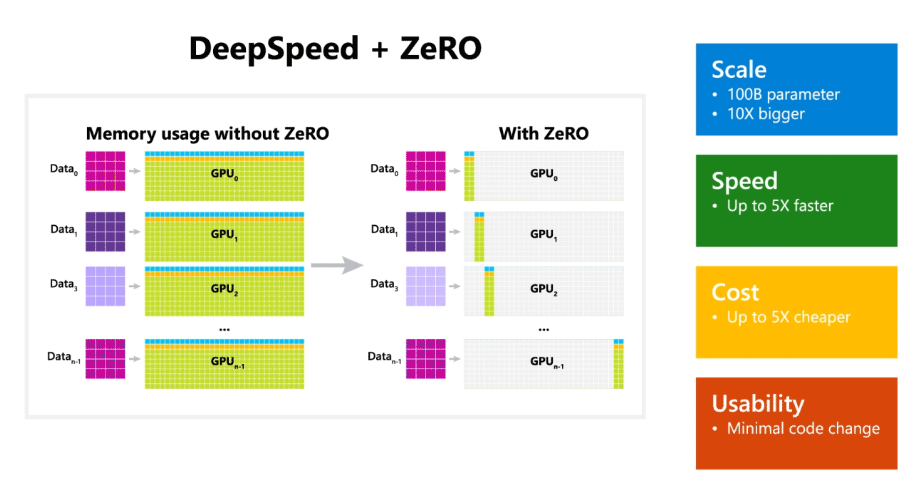
\includegraphics[scale=0.35]{images/tnlg}
	\caption{\emph{T-NLG}, \emph{DeepSpeed} and \emph{ZeRo}.}
	\label{fig:tnlg}
\end{figure}
\paragraph{}
In addition, \emph{T-NLG} has demonstrated that, as large is the \emph{LM} the less of data is needed to learn, improving results of other architectures using less amounts of data. Despite of this, \emph{T-NLG} trained with practically any \emph{dataset} available for different tasks, which gives the model a good knowledge of different domains. This also makes possible for \emph{T-NLG} to use different types of documents, such as \emph{e-mails} or \emph{PowerPoints}.
\paragraph{}
Unfortunately, code has not been released, but the results published by \emph{Microsoft} are encouraging.
\subsubsection{BART}
\noindent \emph{BART} is a model based on the standart architecture \emph{sequence-to-sequence} with \emph{encoder-decoder} layers based on \emph{Transformers}, Figure \ref{fig:bart}\cite{Lewis2019}. Its compound of a \emph{bi-directional encoder} (like \emph{BERT}) followed by a \emph{lef-to-right decoder} (like \emph{GPT}), which allows it to learn the context in a good way (thanks to the \emph{bi-directional encoder}) and to generate high-quality text (thanks to the \emph{left-to-right decoder}).
\begin{figure}[h!]
	\centering
	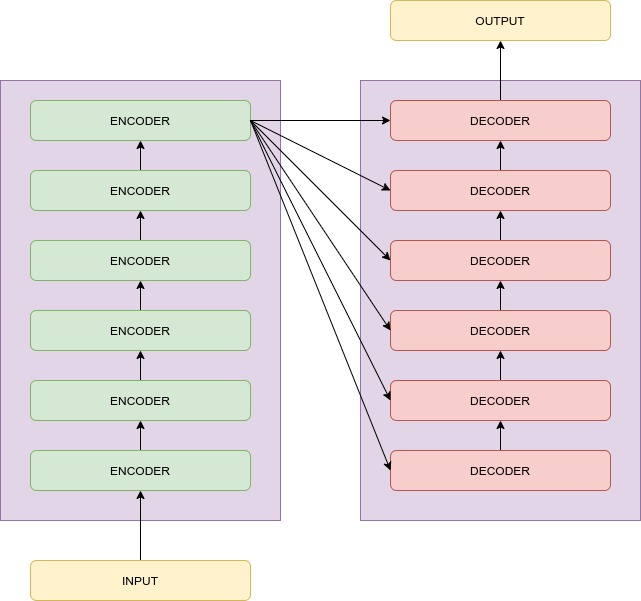
\includegraphics[scale=0.35]{images/bart}
	\caption{\emph{BART} architecture.}
	\label{fig:bart}
\end{figure}
\paragraph{}
The training used for \emph{BART} is based on the mask training used by \emph{BERT} but with a few variations. The model is optimized based on a loss function obtained between the output of the \emph{decoder} and the original text, that is ``corrupted'' with different transformations to make a noised input, forcing the model to capture the language information in an extremly way to understand the noisy input.
\paragraph{}
Among the different ways of ``corrupting'' the text, some of the are:
\begin{itemize}
\item \emph{Token} masking. \\ Same as \emph{BERT}, it masks random \emph{tokens}.
\item \emph{Tokens} removal. \\ In addition to the mask of different \emph{tokens}, \emph{BART} also remove them, thus it has to learn not only to replace the masked \emph{tokens} with the original ones, but also to recognize is some \emph{tokens} are missing and, in that case, to predict which one was the original \emph{token}.
\item \emph{Spans} masking. \\ \emph{BART} not only mask single \emph{tokens}, but also text \emph{spans} are completely masked with a single \emph{[MASK] token}. This way, \emph{BART} has to learn if the mask \emph{token} was a single word or a text \emph{span}. 
\item Sentence permutation. \\ Sentences are randomly shuffled to make the model to learn the real order of the sentences.
\item Document rotation. \\ A random \emph{token} is chosen to rotate the document in a way that it begins with that token, making \emph{BART} to learn to recongize the real start of the document.
\end{itemize}
This way, \emph{BART} trains with highly noised documents and it has to learn to reconstruct them, allowing it to reach a high understanding of the language and to execute different \emph{NLP} tasks, like \emph{QA} or \emph{TS}.
\subsubsection{ProphetNet}
\noindent Another interesting approach is the one proposed by Yan et al.\cite{Yan2020} \emph{ProphetNet} is a novel architecture based also on \emph{encoder-decoder} but, instead of predicting just the next \emph{token} its trained to predict the $n$ next \emph{tokens}.
\paragraph{}
This way, authors say that the overfitting in near words is avoiding as also its the underfitting in far away ones, because in traditional \emph{LM} to predict the next \emph{token} the model focus only on near words, loosing therefore the information provided by \emph{tokens} far away.
\paragraph{}
But in some \emph{NLP} tasks  such \emph{TS} and when dealing with large texts all the context is important for the result, making \emph{ProphetNet} an interesting approach.
\subsubsection{ELECTRA}
Clark et al. propose \emph{ELECTRA} (Efficiency Learning an Encoder that Classifies Tokens Replacements Accurately).\cite{Clark2020} Instead of using the mask training like \emph{BERT} (and so others \emph{LM}), \emph{ELECTRA} uses a novel training way.
\paragraph{}
Instead of replace random \emph{tokens} with a \emph{[MASK] token} (as \emph{MLM} use to do), \emph{ELECTRA} replace them with plausible alternatives by using a ``generator'' (another \emph{MLM}). This way the ``discriminator'' tries to recognize the replaced \emph{tokens}, classifying them as ``original'' or ``replaced'', Figure \ref{fig:electra}. This training reminds to the Generative Adversarial Networks used in Computer Vision tasks, in which two neural networks compete, one of them generates fake images and the other one has to recognize the fake images from a set with real samples.
\begin{figure}[h!]
	\centering
	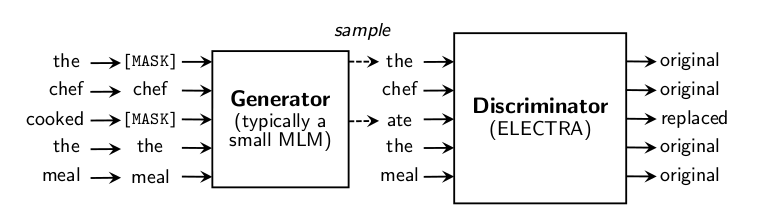
\includegraphics[scale=0.45]{images/electra}
	\caption{\emph{ELECTRA} architecture.}
	\label{fig:electra}
\end{figure}
\paragraph{}
Therefore, \emph{ELECTRA} trains with every single \emph{token} within the document, not only with those that has been masked like the rest of \emph{MLM} do. This makes that \emph{ELECTRA} is able to understand the language before than other \emph{LM} in a more efficient way Figure \ref{fig:compare-electra}.
\begin{figure}[h!]
	\centering
	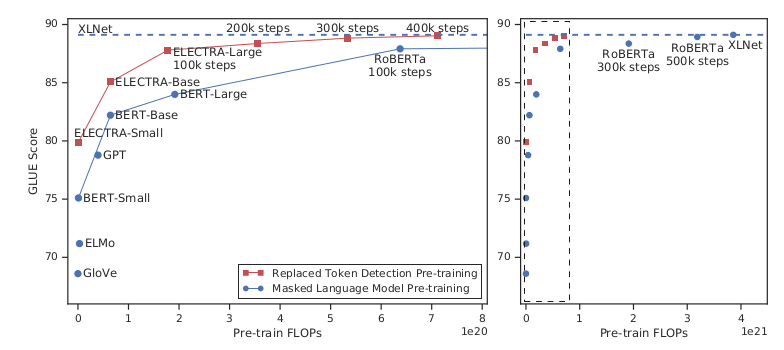
\includegraphics[scale=0.45]{images/compareelectra}
	\caption{Comparison of \emph{ELECTRA} with other \emph{LM}.}
	\label{fig:compare-electra}
\end{figure}
\paragraph{}
This training has allowed that \emph{ELECTRA} reaches state-of-the-art results and, as can be seen in Figure \ref{fig:compare-electra}, in an efficient way. 
\todo{ALBERT}
\todo{LUKE}
\section{Question Answering}
\label{sec:QuestionAnswering}
\noindent Since the begining of the \emph{NLP}, one of the task most studied and researched is the ability to retrieve information based on a simple query, which is know as Information Retrieval (\emph{IR}). This helps people to find any kind of information in the vast amount of data that is being recollected day to day. For example, search engines like \emph{Google}, are not more than a system of \emph{IR} able to find the documents (web pages) that are more related to the query.
\paragraph{}
But most of the time what people wants is not the whole document but a concise answer to a specific question. This is what the Question Answering tries to solve. Given a question over a context, the \emph{QA} systems try to gives an answer to the user. This context use to be a document that could have been retrieved by an \emph{IR} system, but it's only a document, not a collection of them.
\paragraph{}
This has made possible to search engines and intelligent assistants to improve its performance and to understand the user, improving therefore the user experience with this kind of systems. In Figure \ref{fig:google} it can be seen how the search engine \emph{Google} answers a given question with a concise answer.
\begin{figure}[!h]
	\centering
	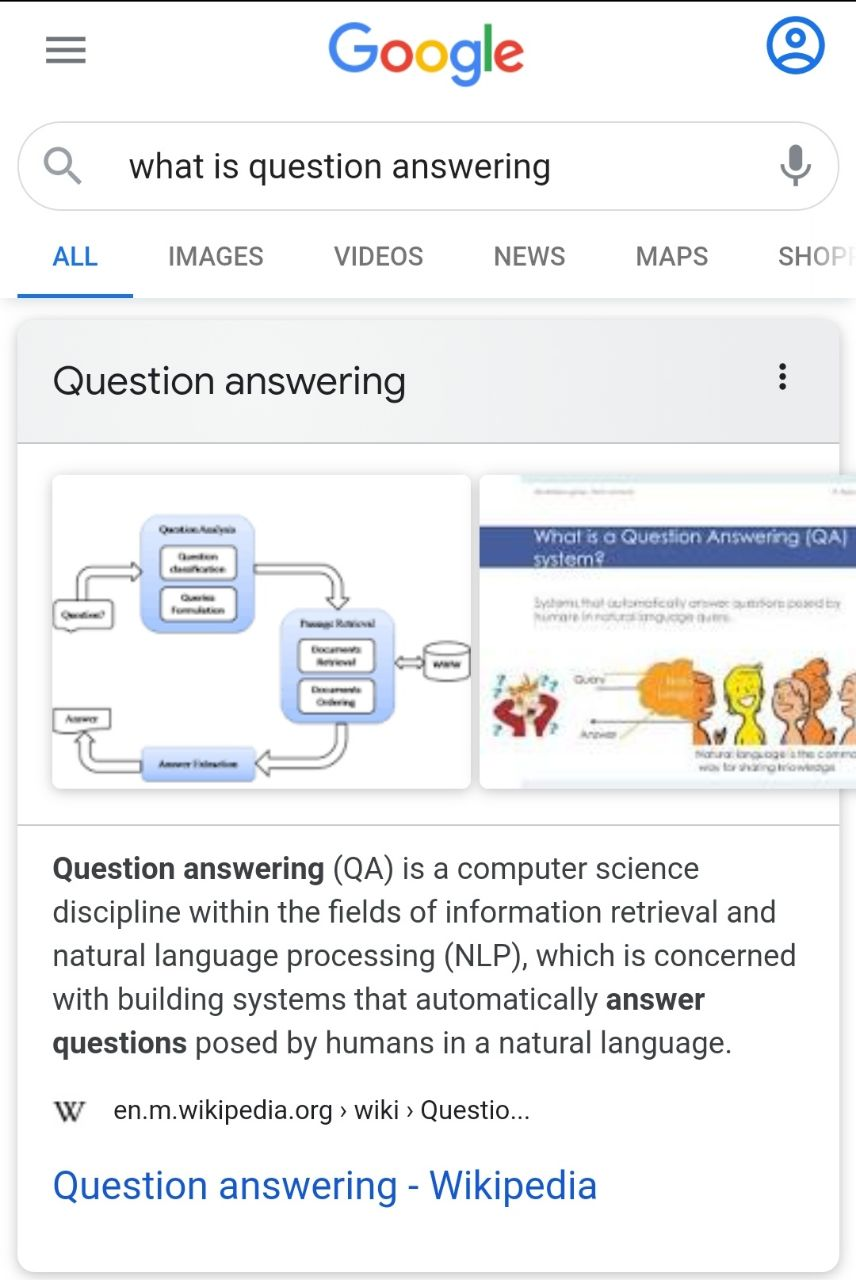
\includegraphics[scale=0.15]{images/google}
	\caption{Question Answering system working in the search engine \emph{Google}.}
	\label{fig:google}
\end{figure}
\paragraph{}
These systems are able to give the answer not only in a written form, but also verbally, and giving also the reference of the document where the answer has been found, in this case \emph{Wikipedia}. As these systems result to be really useful and interesting, both the research and the company fields focused on this task. For instance, the \emph{QA} task was included in the \emph{TREC}, Text REtrieval Conference, or the released of the \emph{Watson} system by \emph{IBM}.
\paragraph{}
Along the history of the \emph{QA} systems there have been proposed different architectures for tese systems, but all of them share some modules that are common in all the systems, as Gonzalez pointed \cite{Gonzalez2003}. These basic modules can be seen in Figure \ref{fig:qa-modules}.
\begin{figure}[!h]
	\centering
	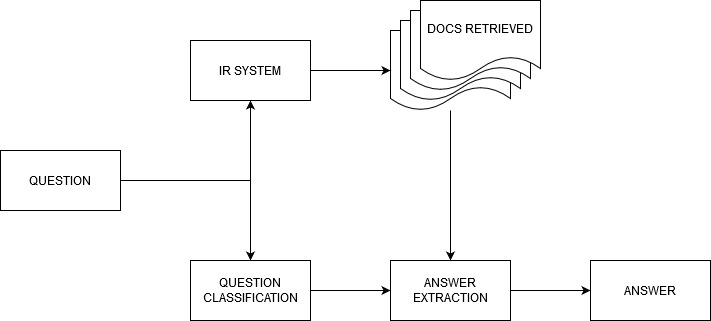
\includegraphics[scale=0.35]{images/qamodules}
	\caption{Question Answering common modules.}
	\label{fig:qa-modules}
\end{figure}
\paragraph{}
The basic workflow in \emph{QA} systems is as follows: 
\begin{enumerate}
\item An \emph{IR} system retrieves the most relevant documents, meanwhile the question is analysed and classified. The question is classified into different types (e.g.: yes/no question, year-expected, etc) to know what kind of answer is expected (a name, a year, an affirmation or negation, etc).
\item Once it is known the type of answer expected by the question and the most relevant documents have been retrieved, the question is searched within each of the documents. If the answer is foud it can be returned to the user or it can be wieghted in case there are more than one answer found.
\end{enumerate} 
\paragraph{}
These modules are expanded (or reduced) in some approaches, like for instance in \cite{Ahmed2016a}, where a sub-module is added to the \emph{IR} module. This new sub-module, the \emph{passage retrieval}, is in charge of retrieve the passage within the document that is related to the question. This way, the \emph{answer extractor} module has to look for the answer not in the whole document, but in the related passages. This can be good, less text means less computational and temporal cost, or bad(less text could mean worse performance, becuase if the \emph{passage retrieval} fails and do not retrieve the passage the answer is located in, the \emph{answer extraction} is not going to be able to find it. But, if the module works as expected, less text will mean also less noise to the \emph{answer extraction} module, which could improve the performance of the system.
\begin{figure}[!h]
	\centering
	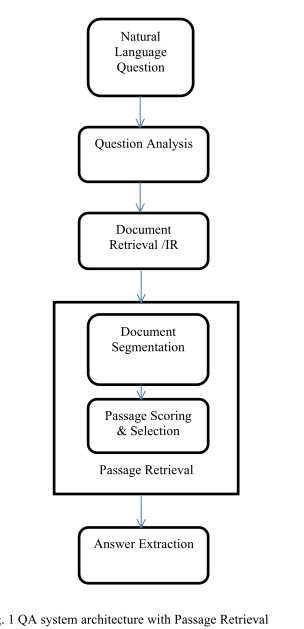
\includegraphics[scale=0.35]{images/ahmed2016}
	\caption{Workflow proposed by Ahmed.}
	\label{fig:ahmed}
\end{figure}
\paragraph{}
This \emph{passage retrieval} module was used in multiple approaches, like the one proposed in \cite{Pablo-Sanchez}, and it was a single task in \emph{TREC} before the \emph{QA} task. 
\paragraph{}
But, with the appearance of the \emph{Transformer} architecture, these modules has changed and modules like \emph{question classification} has even been removed. This module classified the question to know what kind of answer was expected. Along the different \emph{TREC} conferences there have been proposed a los of taxonomies of question and answers types, like the proposed by Moldovan et al. in \cite{Moldovan2001} for the \emph{TREC-8}, the one proposed by Li and Roth for the \emph{TREC-10}\cite{Li2002} or the proposed by Radev et al. in \cite{Radev2005}, Table \ref{tab:radev}.
\begin{table}
	\centering
	\begin{tabular}{|c|c|c|}
		\hline 
		PERSON & PLACE & DATE \\ 
		\hline 
		NUMBER & DEFINITION & ORGANIZATION \\ 
		\hline 
		DESCRIPTION & ABBREVIATION & KNOWNFOR \\ 
		\hline 
		RATE & LENGTH & MONEY \\ 
		\hline 
		REASON & DURATION & PURPOSE \\ 
		\hline 
		NOMINAL & OTHER &  \\ 
		\hline 
	\end{tabular} 
	\caption{Taxonomy proposed by Radev et al.}
	\label{tab:radev}
\end{table}
\paragraph{}
There are also different types of \emph{Question Answering} systems based on the strucutre of the problem. Some of the time the system is given just a document and a question, and it has to look for the answer to the question within the document, extracting the \emph{span} of text that answers the question and this is why these systems are known as \emph{Extractive Question Answering}. 
\paragraph{}
However, sometimes there are a few options and the model has to choose which one is the correct answer to the question, what is known as \emph{Multiple-Choice}.
\paragraph{}
But both of them have the same objective, to find an answer to a question. The first type, the \emph{Extractive QA} has to find for the \emph{span} of text that answers the question. This way, it is able to find the question within the text but, on the other hand, it can only answer with the \emph{span} extracted and it is not able to answer applying \emph{common-sense} and, for instance, they're not able to answer with a ``yes'' or ``no'', they can only extract the span more related to the expected answer by the question.
\paragraph{}
In the second type, the \emph{Multiple-Choice} problems are able to apply some \emph{common-sense}, being able to answer ``yes/no'' questions, relationing countries with cities, languages and so on, but they can only choose between the options given, without being able to find the answer by themselves.
\subsection{Evaluation of QA systems}
\label{sec:qa-evaluation}
The same way that there are different types of \emph{QA} systems, there are also different evaluation metrics. The begining of the \emph{QA} systems can be traced to 1999, when the \emph{TREC-8} has a specific track for \emph{QA}. In this track, competitors had to propose different approaches to give a concise answer to a given question that was chosen from different sources, from question asked by the competitors theirselves to question obtained from the \emph{FAQFinder} system.
\paragraph{}
At the end, the systems were evaluated, in this case a manual evaluation was carried out, this is, were humans the ones that evaluated. As is explained in \cite{Voorhees1999}, several problems were found while evaluating the systems, with even humans doubting about which one was the correct answer.
\paragraph{}
For instance, one of the doubts was if it would be considered as right in questions about a person just the full name, or if the name or the lastname should be considered as right, or if a list of different names is returned, in which the correct name is contained, but the user don't know for sure which one is.
\paragraph{}
Because of this, they came to the conclussion that, to an answer being considered as right, this should answer the question without anydoubt, this is, without having to read the document to know the full answer.
\paragraph{}
Some of the criteria used to consider the answer as right are the next ones:\cite{Allam2012}
\begin{itemize}
\item Relevance: The answer returned should be a response to the question.
\item Correctness: The answer should be factually correct.
\item Concisness: The answer should not contain extraneous or irrelevant information.
\item Completeness: The answer should be cmplete (not a part of the answer).
\item Justification: The answer should be supplied with sufficient context to allow a user to determine why this was chosen as an answer to the question.
\end{itemize}
Based on these concepts the answers are classified into different types, as explained in \cite{Allam2012} and \cite{Pablo-Sanchez}:
\begin{itemize}
\item Correct answer.
\item Failed answer.
\item Inexact answer (irrelevant content or missing data).
\item Unsupported answer (not supported by other documents).
\end{itemize}
With these criteria the doubts commented before are solved, for instance, the fact that the answer is not complete (the problem of the names), the fact that the answer alone must be enough for the user without other sources or that the answer should be concise (for example, not returning a list of multiple names).
\paragraph{}
These evaluation metrics have also evolved and nowadays, eventhough the manual evaluation carried out by humans is still used in some articles, the most common is to evaluate the systems in an automatic way, like the \emph{precission}, the \emph{recall} or the \emph{f1-score}. But other metrics less known have been used, like the ones used in the conferences \emph{TREC-8} and \emph{TREC-11}, the \emph{Mean Reciprocal Rank (MRR)} and the \emph{Confidence Weighted Score (CWS)} respectively, that are defined as:
\begin{equation}
MRR = \sum_{i=1}^{n}\frac{1}{r_{i}}
\label{eq:mrr}
\end{equation}
Where $n$ is the number of questions and $r_{i}$ is the \emph{rank-value} of the first correct answer for the $i$th question.
\begin{equation}
CWS = \sum_{i=1}^{n}\frac{p_{i}}{n}
\label{eq:cws}
\end{equation}
With $n$ being the number of questions and $p_{i}$ the \emph{precission} of the answers from the 1 to the $i$ in a sorted list of answers.
\paragraph{}
Meanwhile the \emph{Multiple-Choice} problems are easily evaluable, because can be treated as classificaction problems, but the \emph{Extractive QA} systems are more complicated to evaluate, because there can be more than one \emph{span} within the text could be a correct answer from the question. Systems also can return the correct labelled \emph{span} but with some added words or without all of them, but being still a correct answer.
\paragraph{}
Anyway, to be able to evaluate these systems in an automatic way, several \emph{datasets} were made.
\subsection{Datasets of QA}
\label{sec:qa-datasets}
\todo{Introduction to QA Datasets}
\subsubsection{SQuAD}
\label{sec:squad}
The \emph{SQuAD} (Sanford QUestion Answering Dataset)\cite{Rajpurkar2016} is a \emph{dataset} created by Rajpurkar et al. in 2016 for \emph{Extractive QA}. It consists of more than 107.785 questions asked over 536 different \emph{Wikipedia} articles by crowdworkers. Given a \emph{Wikipedia} article they have to post a question about the text that the answer is a \emph{span} of text included in the article.
\paragraph{}
To collect the \emph{dataset} the authors used Project Nayuki's \emph{Wikipedia's} internal \emph{PageRanks} to obtain the top 10000 articles of english \emph{Wikipedia}. Then, they select 536 random articles from them and removed figures, tables, short paragraphs, etc. The finally get a set of 23.215 paragraphs for that 536 articles of different topics. Finally they splitted the \emph{dataset} into a training set (80\%), a development set (10\%) and a test set (10\%).
\paragraph{}
Once the articles had been recollected, they employed crowdworkers (like \emph{Amazon Mechanical Turk}) to create the questions and its answers. 
\paragraph{}
Authors then analyzed the question types, the difficulty of the question and the degree of syntactic divergence between the question and the answer. Table \ref{tab:squad-types} shows the different question types and its percentage of appearance in the \emph{dataset}. A complete and official analysis of the \emph{dataset} can be found in \cite{Rajpurkar2016}.
\begin{table}[!h]
	\centering
	\begin{tabular}{|c|c|}
	\hline 
	Answer Type & Percentage (\%) \\ 
	\hline 
	Date  & 8.9\% \\ 
	\hline 
	Other Numeric & 10.9\% \\ 
	\hline 
	Person & 12.9\% \\ 
	\hline 
	Location & 4.4\% \\ 
	\hline 
	Other Entity & 15.3\% \\ 
	\hline 
	Common Noun Phrase & 31.8\% \\ 
	\hline 
	Adjective Phrase & 3.9\% \\ 
	\hline 
	Verb Phrase & 5.5\% \\ 
	\hline 
	Clause & 3.7\% \\ 
	\hline 
	Other & 2.7\% \\ 
	\hline 
	\end{tabular} 
	\caption{Diversity of questions in \emph{SQuAD}.}
	\label{tab:squad-types}
\end{table}
\paragraph{}
To evaluate the systems two different metrics are used over a clean answer (removing punctuation, articles, etc):
\begin{itemize}
	\item Exact match (\emph{EM}): \\
		If the answer matches exactly with any of the ground-truth answers.
	\item \emph{f1-score} (\emph{F1}): \\
		Considering the answer and the ground-truth answers as a bag of words, the \emph{f1-score} is computed between them to measure the average overlap.
\end{itemize}
Authors baseline\cite{Rajpurkar2016} (consisted on window sliding) got a 13.0\% in \emph{EM} and 20\% in \emph{F1} (both of them in test set). A \emph{Logistic Regression} got 40.4\% and 51\% respectively and human performance gets 77\% and 86.8\%.
\paragraph{}
Rightnow, the top \#1 benchmark for \emph{SQuAD} is \emph{LUKE}\cite{Yamada2020} by Yamada et al. that gets a 90.2\% in \emph{EM} and 95.4\% in \emph{F1}.
\paragraph{}
But models trained only on this \emph{dataset} have a problem. If the question is not answerable with the context they make an unreliable response anyway. To solve this \emph{SQuAD} was updated to \emph{SQuADv2}\cite{Rajpurkar2018} with more than 50.000 questions that are indeed not answerable. This way, models have to know when they can answer a question and when they can not.
\paragraph{}
With the same metrics the new human performance is 86.8\% in \emph{EM} and 89.4\% in \emph{F1}. Top \#1 model is \emph{SA-Net on Albert (ensemble)} and gets 90.724\% in \emph{EM} and 93.011\% in \emph{F1}.
\subsubsection{RACE}
\label{sec:race}
\emph{RACE} (Large-scale ReAding Comprehension Dataset From Examinations)\cite{Lai2017} is a \emph{dataset} created by Lai et al. in 2017 for \emph{Multiple-Choice QA}. It consists of near 28.000 passages and near 100.000 questions with 4 possible options each. These questions and passages were collected from english exams for middle and high school chinese students in the age range between 12 to 18. This way, questions were made by english teachers to enhance and measure the english knowledge of the students, so they cover different topics and are designed to require a high level of reading comprehension and reasoning. 
\paragraph{}
As \emph{RACE} covers a wide range of ages (12-18), the authors splitted it into \emph{RACE-M} and \emph{RACE-H}. \emph{RACE-M} denotes the passages and questions collected from the middle schools students (12-15 years old), meanwhile \emph{RACE-H} denotes the ones collected from the high schools students (15-18 years old). Then bot of them were spliited into training set (90\%), development set (5\%) and test set (5\%). Table \ref{tab:race-sets} shows the number of passages and questions in each with a total number of passages of 27.933 and 97.687 different questions.
\begin{table}[!h]
	\begin{tabular}{|c|ccc|ccc|ccc|}
	\hline 
	Dataset &  & \emph{RACE-M} &  &  & \emph{RACE-H} &  &  & \emph{RACE} & \\ 
	\hline 
	Subset & Train & Dev & Test & Train & Dev & Test & Train & Dev & Test \\ 
	\hline 
	\# passages & 6.409 & 368 & 362 & 18.728 & 1.021 & 1.045 & 25.137 & 1.389 & 1.407 \\ 
	\hline 
	\# questions & 25.421 & 1.436 & 1.436 & 62.445 & 3.451 & 3.498 & 87.866 & 4.887 & 4.934 \\ 
	\hline 
	\end{tabular} 
	\caption{Number of passages and questions in each \emph{RACE} set.}
	\label{tab:race-sets}
\end{table}
\paragraph{}
As it can be seen the number of passages and questions is much larger in the \emph{RACE-H} set, the same as the vocabulary size and the length of the passages, questions and options. Altough the vocabulary size is large (136.629), authors note that as the passages and questions have been collected from english exams to chinese students the vocabulary is not as complex as in other \emph{datasets} where data is collected from news, \emph{Wikipedia} or other sources. 
\paragraph{}
To understand the reading comprehension and reasoning required by \emph{RACE} authors analyzed the \emph{dataset} ``classifying'' the questions into:
\begin{itemize}
	\item Word  matching: The  question  exactly matches a span in the article. The answer is self-evident.
	\item Paraphrasing: The question is entailed or paraphrased by exactly one sentence in the passage. The answer can be extracted within the sentence.
	\item Single-sentence reasoning: The answer could be inferred from a single sentence of the article by recognizing incomplete information or conceptual overlap.
	\item Multi-sentence reasoning: The answer must be inferred from synthesizing information distributed across multiple sentences.
	\item Insufficient/Ambiguous: The question has no answer or the answer is not unique based on the given passage.
\end{itemize}
And, more specifically into:
\begin{itemize}
\item Detail reasoning: to answer the question, the agent should be clear about the details of the pas-sage. The answer appears in the passage but it can-not be found by simply matching the question withthe passage. 
\item Whole-picture reasoning: the agent needs to understand the whole picture of the story to obtain the correct answer. 
\item Passage summarization: The question requires the agent to select the best summarization of the passage among four candidate summarizations. 
\item Attitude analysis: The question asks about the opinions/attitudes of the author or a character in the story towards somebody or something
\item World knowledge: Certain external knowledge is needed like simple arithmetic, geography, etc.
\end{itemize}
\paragraph{}
A complete analysis and different methods can be found in \cite{Lai2017}. In the article authors compare human performance with the results of different methods such as windows sliding or \emph{Stanford AR}. The human performance is 95.4\% for \emph{RACE-M} and 94.2\% for \emph{RACE-H}. The top \#1 right now is \emph{Megatron-BERT (ensemble)}\cite{Shoeybi2019} by Shoeybi et al. from \emph{Nvidia}, that achieves an accurcy of 93.1\% for \emph{RACE-H}	and 90.0\% for \emph{RACE-M}.
\subsubsection{QuAIL}
\label{sec:quail}
\emph{QuAIL} (Getting Closer to AI-complete Question Answering: A Set of Prerequisite Real Tasks)\cite{Rogers2020} is a \emph{dataset} created by Rogers et al. in 2020 for \emph{Multiple-Choice QA}. In the article, authors say that altough there are several \emph{datasets} for different reasoning tasks (such \emph{QA}), most of them get ``solved'' almost inmediately, and this is because of the poor diversity of the data, that has bias and spurious patterns that make the models to recognize these patterns more than to actually learn the language. To solve this, the authors have analyzed different \emph{datasets} and have balanced different types of data to try to reduce the amount of bias and spouring patterns.
\paragraph{}
This has led the authors to find that, for instance, paraphrasing makes models to miss performance, even for \emph{BERT} and other \emph{LM}.
\paragraph{}
\emph{QuAIL} is a multi-domain \emph{dataset} with 200 texts for each of the 4 domains available. Questions about these texts have 3 different options and one \emph{Not Enough Information (NEI)} question, that it's the correct option for unanswerable questions. The texts are from 4 different domains: CC license fiction, Voice of America news, blogs and user stories from Quora and each one has 18 question (\~14k questions). The question are classified into the next types:
\begin{itemize}
	\item Text-based questions: Those questions that the information needed to answer should be found in the text.
	\begin{itemize}
		\item Reasoning about factual information in the text.
		\item Temporal order of events.
		\item Character identity.
	\end{itemize}
	\item Word knowledge questions: Those questions that the answer rely on some kind of inference about characters and events, based on information in the text and world knowledge.
	\begin{itemize}
		\item Causality.
		\item Properties and qualities of characters.
		\item Belief states.
		\item Subsequent state after the narrated events.
		\item Duration of events.
	\end{itemize}
	\item Unanswerable questions. 
\end{itemize}
To avoid some possible cooccurence of words the authors performed paraphrasing in a total number of 556 questions of 30 fiction texts, aiming in particular to reduce lexical cooccurrences between the text and the words in the question and the correct answer. Results showed that all models suffered a significant drop in performance, specially for \emph{BERT}.
\paragraph{}
The official benchmark\footnote{\url{http://text-machine.cs.uml.edu/lab2/projects/quail/}} shows tha only the authors have submitted their models, so it's not possible to compare models yet, but the top \#1 of the leaderboard is for the model \emph{TML BERT Baseline} with a 53.4\% for all questions.
\todo{SWAG}
\todo{ARC}
\section{Explainability}
\label{sec:Explainability}
\noindent Deep Learning systems are highly used among society and most of the companies nowadays. These technologies have revolutionized the global thinking of business, allowing to make efficient processes and to solve new tasks unthinkable until now like those involving language understanding. Undoubtedly \emph{AI} systems offer huge benefits and enhance a large number of human activities, however, the use of these systems in some critical business processes like people hiring or credit granting are huge decisions and it is not clear how the model is making these decisions and what are the features in which the model is trusting in order to make the predictions. This way, the effectiveness and insights obtained by the models are limited due to the inability to explain the decisions taken by the models and the repercussion that those decisions may have on the users.
\paragraph{}
This fact has created many concerns about the risks that they introduce and has reduced the initial excitement about the transformation and improvements introduced by these systems. Concerns that have been raised include possible lack of algorithmic fairness (leading to discriminatory decisions), potential manipulation of users, potential lack of inclusiveness, infringement of consumer privacy, and related safety and cybersecurity risks. The use of artificial intelligence explainability (\emph{XAI}) can solve these concerns and provide several business benefits such as:
\begin{itemize}
\item Explanations can help to identify problems in data and features so it can improve the model performance at the same time that can help to better decision making thanks to the additional information provided.
\item Gives a sense of control and safety since the \emph{AI} system owner knows in every moment how the behaviour is and each decision can be subjected to pass through safety guidelines and alerts on its violation.
\item One of the main advantages is the possibility to build trust around the model with the stakeholders who can interpret every decision made. Moreover it can monitor ethical issues and violation due to bias in data.
\item Lastly, it can solve compliance issues related with accountability and regulation. (E.g. Adherence to \emph{GDPR} regulation where ``Right to Explain'' is must-have for a system).
\end{itemize}
\emph{XAI} will take more and more importance and a significant part of the effort from the research community and companies will be focused on creating interpretable models or providing a set of tools that help to understand and explain the decisions taken by the \emph{AI} models. The goal is to enable users to understand, trust model predictions while maintaining the learning performance.
\subsection{XAI classification}
\noindent Altough explainability is a recent technique, there are already a lot of different techniques and systems to try to explain models and predictions. Even tough there a lot of techniques, all are based on the same concepts and, therefore, they can be classified depending on their nature in different aspects:
\paragraph{Global Interpretation vs Local Interpretation} Among the different classifications that can be done in order to difference between all the \emph{XAI} techniques, the most important is the type of the explanation. The are two different types of explanations: the explanation of how a model works and the explanation of why a model has given a specific output as a result. 
\paragraph{}
This way, the \emph{Global Interpreters} try to understand the whole model, how it works and what \emph{features} are important for the model to explain the entire model's predictive reasoning. This is very interesting for some use cases, like for instance to understand if the model has some \emph{bias}. On the other hand, the \emph{Local Interpreters} try to explain a unique prediction of the model, by looking at a local subregion in the feature space around the prediction, trying to understand the model decision based on that local region.
\paragraph{Model-specific vs model-agnostic} Other interesting classification of the \emph{XAI} techniques available is to know which ones can be applied to all models or which ones can only be applied to a specific model type. If, for instance, a company has different models being used (e.g. Support Vector Machines, Random Forests and Neural Networks) its more interesting for the company to use the same tool for all models rather than one different technique for each one. Model-specific tools are those one that can be only applied to a specific model type (for instance, those tools that study the \emph{attention} mechanism can only be applied to language models that use \emph{attention}). Model-agnostic, on the other hand, are those tools that can explain every model, no matter its type.
\paragraph{Intrinsic vs post hoc} Simple machine learning models can be explained themselves, this interpretability is considered as intrinsic e.g. rules-based, linear models, parametric models or tree based models. In these types of models the explanation arise itself with the output of the model, and there is no need of post processing to generate an explanation. However, complex models such as Neural Networks require some additional processing to be performed after the predictions are made in order to get the explanation.
\subsection{XAI Techniques}
\noindent Altough there are a lot of different techniques available to explain models or predictions, there are some techniques that are the most frequent in the literature. Most of the available tools for \emph{XAI} use these techniques to give the explanation.
	\paragraph{Feature Importance} The model generates the output by performing operations over the inputs, this is, the \emph{features}. Therefore, to understand the importance of the \emph{features} can help to understand the model beahaviour and to explain it.
	\paragraph{Surrogate Model} If the type of the model is not easily interpretable (such as Neural Networks) or if it is not known, a common way to explain it is to build a second model easily explanaible, that will try to behave exactly the way that the model to explain does. This way, by explaining the second model the first one can be explained.
	\paragraph{Example-Driven} This technique is based on search for a similar labeled instance to the input, that will be used as an explanation. These similar instances are obtained from labeled data and they can be gotten by studying semantic similarity, or nearest neighbors in the \emph{feature} space.
	\paragraph{Provenance} In some systems the prediction process involves a series a of reasoning steps, in this cases, the prediction steps can be illustrated to be used as explanation.
	\paragraph{Induction} Some way to explain the model functioning is to generate human-readable representations, such as rules or decission trees that are induced as explanations.
	\paragraph{Anchors} Models use to have some bias in the traning data (and therefore in themselves). There are also some inputs that condition an specific output in a way that, if input $x$ is present, the output is always going to be $o$. This is known as an \emph{anchor} and this technique looks for anchors to help to understand a local prediction.
\paragraph{}
These techniques are all based in solving a few operation that enable explainability. Although some of them depend on the type of model being used (\emph{model-specific}, other are applied to any kind of architecture (\emph{model-agnostic}) such as the \emph{Surrogate Model} technique, that usually is trained with \emph{perturbations of the input}\cite{Ribeiro2016} mades by generating random instances modifiying the input $x$. Another technique that can be used with different types of models (althoug it is mostly used with \emph{NN}) is the \emph{first-derivative saliency}, which consists on ``estimate the contribution of input $i$ towards output $o$ by compuing the artial derivative of $o$ with respect to $i$''.\cite{Danilevsky2020}
\paragraph{}
On the other hand, the \emph{model-specific} techniques use to involve some particularities of the model. For instance, if using \emph{RNN}, and more specifically \emph{LSTM}, the output of the \emph{LSTM} cells and the output of the ``gates'' within them can be used to explain the outputs of the model (\emph{Feature Importance} technique, \cite{Ghaeini2018}). More recently, if using \emph{LM} based on \emph{transformers} and/or \emph{attention} layers, the information provided by these layers can be used to explain the behaviour of the model, and because of this there are plenty of works that made use of this startegy, \cite{Luo2018}, \cite{Xie2017}, \cite{Serrano2019}, \cite{Jain2019}.
\subsection{XAI Visualization}
\noindent The main point of \emph{XAI} is to help users and developers to understand the output of a model, why that prediction, why not another one or whay can be done to improve the model performance. So, a really important point is to understand the \emph{XAI} techniques outputs, because if the user does not understand the explanation it's not possible that he understands the model behaviour. 
\paragraph{}
Because of this, the \emph{XAI} visualization is as important as the techniques used to get the explanation and, therefore, there are a lot of different ways of visualize explanatios, depending on the type of the technique used, the model, the kind of the problem (\emph{NLP}, tabular data, computer vision, classification, regression, etc). 
\paragraph{}
\begin{figure}[h]
\centering
\begin{subfigure}{0.3\textwidth}
  \centering
	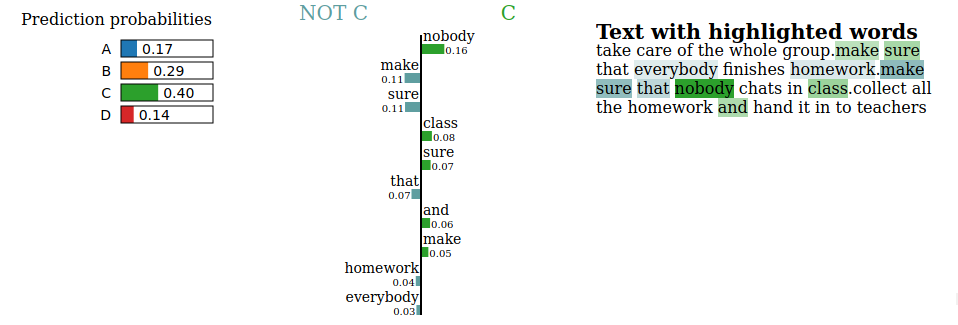
\includegraphics[width=200px]{images/lime-result-2a}
	\caption{Visualization of \emph{LIME}.}
	\label{fig:vis-lime}
\end{subfigure}
\medskip\\
\begin{subfigure}{0.3\textwidth}
  \centering
	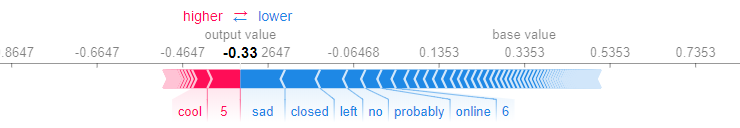
\includegraphics[width=240px]{images/shap}
	\caption{Visualization of \emph{SHAP}.}
	\label{fig:vis-shap}
\end{subfigure}
\medskip\\
\begin{subfigure}{0.45\textwidth}
  \centering
	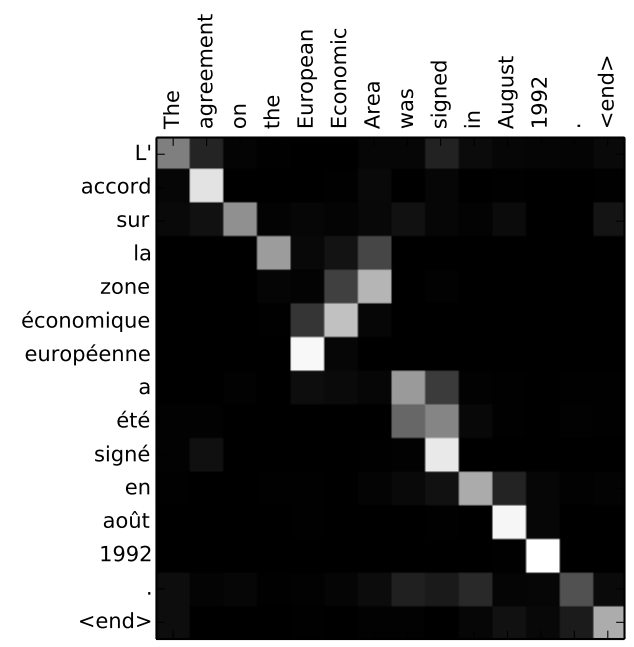
\includegraphics[width=120px]{images/attention}
	\caption{Attention Visualization}
	\label{fig:vis-att}
\end{subfigure}
\begin{subfigure}{0.45\textwidth}
  \centering
	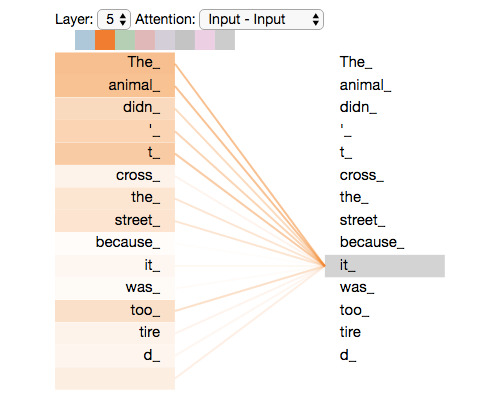
\includegraphics[width=120px]{images/selfattention}
	\caption{\emph{BertVIZ} Visualization.}
	\label{fig:vis-bertviz}
\end{subfigure}
\caption{\emph{XAI} Visualization examples.}
\label{fig:vis-examples}
\end{figure}

\subsection{XAI Evaluation}
\noindent Due to the young age of the \emph{XAI} techniques and to the difficult of the problem being treated, there is no a standard way to evaluate the \emph{XAI} systems and techniques. Most of the papers in the literature that present solutions \cite{Xie2017} don't evaluate the systems and just present a simple discussion and explanation of the \emph{XAI} results based on what the authors think, using only selected examples and not evaluating the system at its whole.
\paragraph{}
Some approaches try to solve this by generating ground truth evaluations to quantify the performance of the \emph{XAI} techniques, by using well known evaluation metrics such as \emph{Precission, Recall and F1-Score}\cite{Carton2018} or \emph{BLEU}\cite{Ling2017}, \cite{Rajani2019}. Although is an interesting way to evaluate the systems, usually there is no only a valid \emph{XAI} explanation, but different explanations may be valid. Because of this, the ground truth aquisition is critic to get a valid evaluation.
\paragraph{}
Other approaches try to solve the problem of multiple valid explanations by using human evaluation. This way, humans can evaluate the quality of the explanations without having to generate ground truth or to measure the similarity of the explanations. This is also interesting, because \emph{XAI} systems try to explain the behaviour of a machine learning model, and this is usually a black box humans don't understand and, therefore, can not generate a real ground truth. 
\paragraph{}
Also, as said before, one important step of the \emph{XAI} pipeline is the visualization, and a \emph{XAI} system that can explain the result better to the user is more effective than another one that does not gives a good visualization for explanations understanding, even if this last one has a greater explanation of the model behaviour. This way, the explanations can be evaluated by its understanding of the model prediction and by the human comprehension of the explanations. Lertvittayakumjorn et al. \cite{Lertvittayakumjorn2019} present three different ways of evaluate the \emph{XAI} systems based on the different goals of these systems: To reveal accurately the model behaviour; to explain the model predictions; to assist humans in future investigations about uncertain predctions.
\paragraph{}
As \emph{XAI} systems effectiveness depends on the human understanding, is important to have multiple evaluators to deal with different responses and subjectivity, like did Sydorova et al. \cite{Sydorova2019}, where 25 humans evaluated and compared explanations of different techniques.
\paragraph{}
One way mostly used to evaluate the explanations of \emph{attention} layers is to set to zero the maximal entry of the layer to see if the prediction is altered \cite{Serrano2019}. This way, if the result is altered by turning off the dominant weights, this would mean that the weights are indeed explaining the result. Same can be applied to other methods, for instance the replacement of the most important words for a specific prediction could change the result if that are actually important words for the prediction.
\section{Explainabity in NLP}
\label{sec:ExplainabilityNLP}
\noindent The same that has happened with other types of \emph{AI} problems, such as time series regression or in computer vision, has happened to \emph{NLP}, this is, the usage of \emph{Deep Learning} to improve the quality and the results of the models and, with it, the lack of explainability.
\paragraph{}
At the beginning, \emph{NLP} models where mainly based in \emph{white box} techniques, such as \emph{Hidden Markov Models (HMM)}, \emph{Decission Trees} or \emph{Logistic Regressions} which are inherently explainable, but with the arrival and popularity of \emph{Deep Learning} models and \emph{word embeddings} as features, it has become almost impossible to understand why a model gives an output instead of another one. 
\paragraph{}
Because of this, many researchers and companies have focused their research in the explainability, and its application to the \emph{NLP} field, developing systems that are able to explain the model behaviour and which features (or word, in case of \emph{NLP}) are more important for the model prediction. But, eventough explainability in \emph{Deep Learning} models is difficult \emph{per se}, and more in \emph{NLP} problems, sometimes it gets even more difficult depending on the problem type.
\paragraph{}
Some \emph{NLP} problems are more complex than others. For instance, text classification problems are less complex than text summarization (depending, of course, on the use case). This is because sometimes there are some words that only appears in some classes, so if that words appear in the text it can be classified without understanding the language. Same happens with simple named entity recognition, where some features like prepositions before the entity, the uppercase and so on help a lot to recognize a named entity. But some problems, like text summarization and question answering are more complex tasks in which the model has to understand the language and the text to be able to solve the task.
\paragraph{}
To understad the language is something really difficult and only humans can do, a lot philosophers say that is language what separates humans from animals actually, and, of course, its complex for machines also. Meanwhile machines are grater than humans while treating with numbers, they can not understand languages as well as humans do, due to the complexity of the task, that involves not only to understand words and grammar, but also to have an understanding about the world, science, politics, history, etc. This makes some tasks really difficult and, although some models have achieved a really good result in some of this tasks, it is not clear if it is because these models understand the language and the task or if it is due to an overfitting. This can be seen in text summarization, where models trained over scientific papers or over news can not summarize other texts with the same performance, giving as output short sentnces (in case of models trained over news), that are not always a good summary.
\paragraph{}
This is why \emph{XAI} is difficult in \emph{NLP} tasks, but also this makes \emph{XAI} important, because if users don't know why the model has given an outuput, they can not trust in it. However, researcher have been working in explain \emph{NLP} models for the last 5 years, developing really good approaches.
\paragraph{}
In 2015 Voskarides et al.\cite{Voskarides2015} use a two-step approach for automatically explaining relationships between entity pairs, selecting sentences that explain the triplets and using machine learning to rank them according to how they explain the relationship between the entities. Other researchers has also pointed out the utility of applying knowledge graph to deep learning models to increase not only the performance but also the explainability of the models \cite{Palmonari2020}, \cite{Lecue2020}. In 2019, Moon et al. presented \emph{OpenDialKG}\cite{Moon2019}, that use knowledge graph to create a dialogue and reasoning system, that also generates a walk path, providing a way to explain conversational reasoning. 
\paragraph{}
But, although there are a few papers explaining others types of systems such as machine learning algorithms, \cite{Pappas2014}, most of the papers with model-specific techniques are focused on the neural networks due to the difficulty to explain them and their great performance. Gupta et al. proposed a technique named as \emph{Layer-wIse-Semantic-Accumulation (LISA)}, \cite{Gupta2018} for explaining RNN, detecting patterns on while decision making. Poerner et al. developed a method called \emph{LIMSSE}, an adaption of \emph{LIME} to NLP, that achieves good performance in NLP and DNN. Something like that did Wallace et al. \cite{Wallace2018}, using \emph{Deep k-Nearest Neighbors}\cite{Papernot2018} for text classification. As they say in the article, the confidence of neural networks is not a robust measure of model uncertainty, making local interpretation methods less robust in these cases.
\paragraph{}
In 2016, Lei et al. proposed a framework in which they used and encoder and a generator to solve the problem \cite{Lei2016}. The idea is to generate \emph{rationales}, that are pieces of input text as justifications, that once they are feed to the encoder the result of the prediction is the same but that they can help to justify the decission. 
\paragraph{}
Alvarez-Melis et al. proposed a framework to explain black-box models based on input perturbation that returns as explanation a set of input-output tokens that are related to each other inside the model \cite{Alvarez2017}. Input perturbation is one of the techniques most used in \emph{XAI}, but Alvarez-Melis et al. proposed a novel way of generatin these perturbations, by using a variational autoencoder to generate similar sentences and, therefore, controlled perturbations. 
\paragraph{}
Another interesting approach is that proposed by Rajani et al. in \cite{Rajani2019}, in which they develop a system named Commonsense Auto-Generated Explanation (\emph{CAGE}) to generate explanations in natural language, by training a model (\emph{GPT-2}) on a new \emph{dataset} called Common Sense Explanations (\emph{CoS-E}).
\todo{Survey of XAI in QA}

\section{Explainability tools}
\label{sec:tools}
\noindent 
\subsection{LIME}
\label{sec:Lime}
\noindent \emph{LIME} (Local Interpretations Model-Agnostic Explanations) is a method developed by \emph{Marco Tulio Ribeiro} to explain any black box classifier, with two or more classes.
\paragraph{}
It's able to explain local predictions of almost any machine learning problem, no matter is a computer vision problem, a \emph{NLP} problem or a problem based on tabular data. As it's model-agnostic it's also able to explain every single algorithm, as it considers the model as a black box. 
\paragraph{}
The implementation of this method is available in the \emph{GitHub} of the author \footnote{\url{https://github.com/marcotcr/lime}} with a \emph{BSD-2 Clause license}, so everyone can use the method. This has made this method very famous, being very used by the community. 
The usage of the tool is very easy. Users have to implement a function that takes as input a \emph{NumPy} array with instances and outputs the result of the prediction, with the probability for each class.
 
\paragraph{Advantages:}
\begin{itemize}
	\item Model-agnostic: It can explain any machine/deep learning model.
	\item Easy visualization.
	\item Fast computation.
\end{itemize}
\paragraph{Disadvantages:}
\begin{itemize}
	\item Local: \emph{LIME} is just local explainer, it cannot explain the entire model behavior.
	\item Randomness: score can be different every time as it generates samples randomly so it lacks of consistency.
\end{itemize}

\paragraph{Method Description} This algorithm takes the assumption that is possible to fit a simple interpretable model around a single observation that will mimic how the global model behaves at that locality. This is what makes \emph{LIME} a model-agnostic method, as it will explain the new model created, which is an interpretable model (\emph{RIDGE}), regardless the type of the model to be explained.
\paragraph{}
It works by perturbing the input and seeing how the predictions change for each perturbed input. It first generates a neighborhood data by randomly hiding features (words in this case) from the text instance.  Then, it generates an explanation by approximating the underlying model by an interpretable one learned on the perturbations of the original instance (e.g., removing words).
\paragraph{}
This way, it learns locally weighted linear models on this neighborhood data to explain each of the classes in an interpretable way and indicate the impact of word existence.
\paragraph{}
\begin{figure}
	\centering
	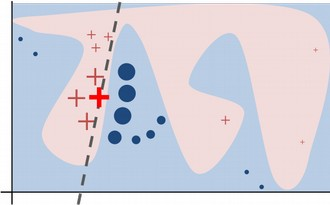
\includegraphics[scale=0.55]{images/lime-explanation}
	\caption{Functioning of \emph{LIME}.}
	\label{fig:lime-ex}
\end{figure}
In the Figure \ref{fig:lime-ex}, the blue/pink background corresponds to the non-linear model being used in the predictions, that has two labels, crosses and circles. While explaining a local predictions (the red cross), \emph{LIME} generates random samples and weights them according to the distance to the prediction being explained (the size of the crosses/circles). The dashes line correspond to the linear model created by \emph{LIME} and its the one being actually explained by \emph{LIME}.

\paragraph{Application to Language Models}
As \emph{LIME} is a model-agnostic method, it's able to explain every type of model, included Language Models. \emph{LIME} is going to consider the original Language Model a black box, creating an additional model, fitted with perturbations of the input. This way, is able to interpret local predictions of Language Models. The perturbations will be made over the instance of the local prediction by, for instance, removing words. 
\paragraph{}
Language Models are based on the prediction of the next word (or sequence), which is more like a regression problem. Even when \emph{LIME} is also able to explain regression problems, is more focused on the classification problems. Nevertheless, the most of the Language Models used nowadays aren't used to predict the next sequence, but to do complex NLP tasks, such as text classification, Named Entity Recognition or Question Answering, and this is done by adding additional layers at the top of the model. This layers will be different depending on the kind of the problem, but most of them can be treated as classification problems. For instance, the Named Entity Recognition problem consists on classify each token as a named entity or not.  This way, \emph{LIME} could be used not only to explain the Language Models themselves, but also the complex model built on top of them, such as \emph{BERT}.

\paragraph{Application to Question Answering}
Question Answering models can be classified into two different types. The ones that try to extract the answer directly from the text, given as the result the tokens inside the text that answer the question (with datasets such as \emph{SQuAD}) and the ones that try to select the correct answer among the possible answers given, which are known also as Multiple-Choice problems (with datasets such as \emph{RACE}).
\paragraph{} 
Depending on the QA type (extractive or multiple-choice) the way to proceed is different, but both of them can be treated as classification problems. In the extractive ones, span classification layer is added on top on the base model (such as \emph{BERT}), and in the multiple-choice ones  a classification layer is added on top of the pooled output to classify which one is the correct answer.
\paragraph{}
This way, considering the QA problem as a classification one, is easy to adapt \emph{LIME} to use it in this kind of tasks. In these cases, \emph{LIME} can take as input the context, the question, the options or any combination possible between them, explaining for instance which words are important of every single option.
\chapter{Methodology}
\fancyhead[RE]{\textsc{Chapter} \thechapter. Methodology}
\label{ch:Methodology}
\noindent The proposal of this work is to review the state of the art of \emph{XAI} of \emph{LM} applied to multiple choice problems. In this chapter the methodology followed is explained.
\section{Description}
\label{sec:Description}
\noindent In order to test the different \emph{XAI} tools, a language model for a multiple choice problem is needed. So the first step covered is to train a \emph{LM} to be used. Then the different \emph{XAI} tools to be tested are going to be adapted to multiple choice problems.
\section{Model Training}
\label{sec:Model training}
\noindent As said before, a language model was trained for a multiple choice problem. Although it is not the best choice for a real problem (nor the one that has the best performance nor the fastest model), \emph{BERT} has been chosen, because it is the most famous language model. 
\paragraph{}
Therefore, a \emph{BERT} model is going to be trained over one of the multiple choice \emph{datasets} seen in Section 2.2.2. The \emph{dataset} selected was \emph{RACE}, taken from the Huggingface \emph{datasets} library. \footnote{\url{https://huggingface.co/docs/datasets/}}. 
\paragraph{}
The implementation of \emph{BERT} used was the one available at the Huggingface \emph{transformers} library. \footnote{\url{https://huggingface.co/transformers/}} Due to hardware limitations the \emph{BERT base} version was used, and as it is not as powerful as the largest version, the \emph{RACE-middle} version of the \emph{dataset} was used. The accuracy obtained after 3 epochs was of $0.641$. Although it could be improved, the goal of this work is not to train a good model for the multiple choice problem but to explain the model decisions, both right and wrong. The code to train the model can be found in:
\begin{itemize}
	\item GitHub: \url{https://github.com/marmg/TFM/blob/main/BERT-RACE.ipynb}
	\item Google Collab: \url{https://colab.research.google.com/drive/1RexG8T8Rz8QvVkX0H-K5VaXpuSY-mAEJ?usp=sharing}
\end{itemize}

\subsection{Explainability model-agnostic}
\label{sec:ModelAgnostic}
\noindent As seen in \ref{sec:xai-classification}, there are different types of \emph{XAI} tools. In this work both model-agnostic and model-specific tools are going to be tested. The probably most famous \emph{XAI} tool is \emph{LIME}, and therefore is going to be tested.
\subsubsection{LIME}
\label{sec:Lime}
\noindent In order to use \emph{LIME} with \emph{BERT} for Multiple-Choice (the same as with any other model), a function has to be developed that takes as input a list of perturbed instances, makes the prediction and return the probability for each class. 
\paragraph{}
Even when is not the efficient, the easiest and most common way to fit the model is by repeating the article, joined to the question and one of the options, for instance while predicting in \emph{RACE} dataset, the result would be four instances with the same article and the same question, but with a different option each. 
\paragraph{}
So, for developing the function used by \emph{LIME}, this four instances have to be created inside it with the perturbations made by the method. Depending on the experiment, this instances will be different because the perturbations will be just the question, the article, the options and so on, and will be concatenated with the original parts that are not being perturbed.
\paragraph{}
Then, the instances are converted to the features to make the prediction. The result is transformed with a \emph{Softmax} function and finally is returned to \emph{LIME}, which analyzes the outputs related to the perturbations made, given as the result a score based on the importance of the word for the prediction.
\paragraph{}
\emph{LIME} works by perturbing the instance to measure the importance of the words, that is enough for most of the \emph{NLP} tasks such as Text Classification. But in Multiple-Choice task there are different parts to take into account, the article or context, the question and the options. Thus, four experiments are going to be made to explore each of the parts.
\begin{enumerate}
	\item 1st experiment: The question is going to be perturbed.
	\item 2nd experiment: The options are going to be perturbed.
	\item 3rd experiment: The article is going to be perturbed.
	\item 4th experiment: The question and the options are going to be perturbed.
\end{enumerate}
With this, not only the most important words are expected to be detected, but also which part is more important for the model.
\paragraph{}
As \emph{LIME} takes as input the instance to perturb and the prediction function, different functions have to be developed in order to make the experiments. One of them will take as input the question and will generate the features of the example by using the original article and options.Other will take as input the options and once again will generate the features of the example by using the original article and, in this case, the original question. The same with the article and with the question and options together. 
\paragraph{}
When there are more than one instance (like in the options), they are going to be concatenated with a special character and the function will split it to generate the different examples.

\subsection{Explainability model-specific}
\label{sec:ModelSpecific} 
\noindent Among the different model-specific options available to study the \emph{LM}, the most famous and useful is to look at the \emph{Attention} weights. \emph{Attention} is used to vectorize the words generating contextual embeddings, taking into account how words relate themselves and what words are in the text to understand the real meaning of the words.
\paragraph{}
This way, to look at the \emph{Attention} has proved to be useful to understand the model behaviour and to be able to prune heads of the \emph{LM}, reducing the size of the model, the time or the hardware needed and, therefore, several tools have been developed to study and to look at the \emph{Attention} layers.

\subsubsection{Attention Heatmap}
\label{sec:AttentionHeatmap}
\noindent The \emph{attention} heatmap is a correlation plot that show hot \emph{tokens} in one sentence attend to \emph{tokens} in other (or the same) sentence. As this only depends on the \emph{tokens} and values that are shown, it is possible to plot a heatmap of \emph{Multiple Choice} and \emph{QA} problems, showing how \emph{tokens} at question attend to \emph{tokens} at options.

\subsubsection{BertViz}
\label{sec:Bertviz}
\noindent Although \emph{BertViz} does not support \emph{QA} or \emph{Multiple Choice} problems by default, it is possible to apply it to these types of problems by modifying the source code, which is open and available in GitHub\footnote{\url{https://github.com/jessevig/bertviz}}.
\paragraph{}
\emph{BertViz} takes as input the \emph{attention} weights and use them to draw the correlation between \emph{tokens} based on these values. Thus, if the \emph{attention} values of a \emph{Multiple Choice} problem is taken as input and it is parsed it is possible to adapt the tool for these problems. The modifications done format the \emph{attention} values to show how \emph{tokens} at question attend to \emph{tokens} at each of the options and vice versa.

\subsection{Intrinsic GPT-3}
\label{sec:gpt3}
\noindent Following the idea of Rajani et al. \cite{Rajani2019} and trying to take advantage of the power of \emph{GPT-3}, one test was developed in order to see if \emph{GPT-3} was able to explain itself. 
\paragraph{}
To force \emph{GPT-3} to generate the explanations (or any expected result), first a few examples of what is exactly desired have to be feed to the model in order to show it what is expected. In this case the model is going to be feed with some examples following the next structure:
\begin{itemize}
	\item Context
	\item Question
	\item Options: Options formatted with an identifier (A-D).
	\item Answer: Identifier of the option chosen. 
	\item Explanation: Explanation of the answer
\end{itemize}
In Appendix \ref{ch:GPT3-Examples} the examples used are shown.
\paragraph{}

%%%%%%%%%%%%%%%%%%%%%%%%%%%%%%%%%%%%%%%%%%%%%%%%%%%
%%% EVALUACION
%%%%%%%%%%%%%%%%%%%%%%%%%%%%%%%%%%%%%%%%%%%%%%%%%%%

\chapter{Results}
\fancyhead[RE]{\textsc{Chapter} \thechapter. Results}
\label{ch:Results}
\noindent Before going deeper into the results, the experiments and examples used to test the tools are being introduced. As tools are different depending to its nature (model agnostic vs model specific), different experiments have to be done.
\paragraph{}
\label{ex:intro}
Besides this, examples used are going to be the same to be able to compare the results. 3 examples of the \emph{RACE test set} have been selected and modified to test the tools. The original examples selected and the modifications are listed below. The part of the article where the answer is appears in bold.
\paragraph{Example 1}
\label{ex:1}
\begin{passage}[Article of Example 1]{art:1}
Take a class at Dulangkou School, and you'll see lots of things different from other schools, You can see the desks are not in rows and students sit in groups. They put their desks together so they're facing each other. How can they see the blackboard? There are three blackboards on the three walls of the classroom! \\
The school calls the new way of learning ``Tuantuanzuo'', meaning sitting in groups. Wei Liying, a Junior 3 teacher, said it was to give students more chances to communicate. \\
Each group has five or six students, according to Wei, and they play different roles .There is a team leader who takes care of the whole group. There is a ``study leader'' who makes sure that everyone finishes their homework. \textbf{And there is a discipline leader who makes sure that nobody chats in class}. \\
Wang Lin is a team leader. The 15-year-old said that having to deal with so many things was tiring. \\
``I just looked after my own business before,''said Wang. ``But now I have to think about my five group members.'' \\
But Wang has got used to it and can see the benefits now. \\
``I used to speak too little. But being a team leader means you have to talk a lot. You could even call me an excellent speaker today.'' \\
Zhang Qi, 16, was weak in English. She used to get about 70 in English tests. But in a recent test, Zhang got a grade of more than 80.\\
``I rarely  asked others when I had problems with my English tests. But now I can ask the team leader or study leader. They are really helpful.''
\end{passage}
Question: ``\emph{A discipline leader is supposed to  \_  .}''\\
Options: 
\begin{itemize}
 \item A: take care of the whole group.
 \item B: make sure that everybody finishes work
 \item C: make sure that nobody chats in class
 \item D: collect all the homework and hand it in to teachers
\end{itemize}
Correct Answer: C. \\ 
Prediction: B. \\
\textbf{$\bullet$ Modification $a$:} \\
Description of the modification: Question paraphrased.\\
New question: \emph{What is a discipline leader supposed to?} \\
Prediction: B. \\
\textbf{$\bullet$ Modification $b$:} \\
Description of the modification: Question and options paraphrased.\\
New question: \emph{What is a discipline leader?} \\
New options:
\begin{itemize}
 \item A: A person supposed to take care of the whole group
 \item B: A person supposed to make sure that everybody finishes work
 \item C: A person supposed to make sure that nobody chats in class
 \item D: A person supposed to collect all the homework and hand it in to teachers
\end{itemize}
Prediction: B. \\
\textbf{$\bullet$ Modification $c$:} \\
Description of the modification: Question paraphrased and changed with a synonym and options paraphrased.\\
New question: \emph{What is an orderliness leader?} \\
New options:
\begin{itemize}
 \item A: A person supposed to take care of the whole group
 \item B: A person supposed to make sure that everybody finishes work
 \item C: A person supposed to make sure that nobody chats in class
 \item D: A person supposed to collect all the homework and hand it in to teachers
\end{itemize}
Prediction: B.
\paragraph{Example 2}
\label{ex:2}
\begin{passage}
A traveler came out of the airport. There were a lot of taxis. He asked every taxi driver about his name. Then he took the third one. It cost 5 dollars from the airport to the hotel. ``How much does it cost for the whole day?'' The man asked. ``100 dollars,'' said the taxi driver. This was very dear, but the man said it was OK. \\
The taxi driver took the man everywhere. He showed him all the parks and museums in the city. In the evening they went back to the hotel. The traveler gave the taxi driver 100 dollars and said, ``What about tomorrow?'' The taxi driver looked at the man and said, ``Tomorrow is another 100 dollars.'' And the man said, ``That's OK! See you tomorrow.'' The taxi driver was very pleased. \\
The next day the taxi driver took the traveler everywhere again. They visited all the parks and museums again. And in the evening they went back to the hotel. The man gave the taxi driver 100 dollars again and said, ``I'm going home tomorrow.'' The driver was sorry because he liked the traveler and 100 dollars a day was a lot of money. ``So you are going home. Where do you come from?'' He asked. ``I come from New York.'' ``New York,'' the taxi driver said, ``I have a sister in New York. Her name is Susan. Do you know her?'' ``Of course I know her. She gave me 200 dollars for you!'' \\
\end{passage}
Question: ``\emph{Where did the traveler come from?}''\\
Options: 
\begin{itemize}
 \item A: America
 \item B: England
 \item C: Canada
 \item D: France
\end{itemize}
Correct answer: A. \\
Prediction: \\
\section{Model-agnostic experiments}
\label{sec:ModelAgnosticExperiments}
\noindent Most of the model agnostic tools are based on instance perturbation, to train an underlying model easily interpretable that emulates the \emph{LM} results.
\paragraph{}
Four different experiments have been developed to test the model agnostic tools and to try to understand which parts are more important for the model in order to make its prediction.
\begin{enumerate}
	\item The first one was based on perturb just the question. \\
	The first idea was to try to explain which words of the question are important for the prediction, because at the end the model has to take as input the question and look for the answer. This way, the question the user asks to the model will determine the result of the prediction, and to know which words of the question are important is a good way to know how to make good questions.
	\item In the second one, the options given to the model were perturbed. \\
	After the question, the most important part on the multiple-choice problems is the set of options given to the model, because it has to choose between some of this options.
	\item The third one consisted on perturb the article. \\
	After all, the model has to look for the answer in the article, so it is important to that the model understands it. Thus, in the third experiment the article was perturbed.
	\item In the final one, both the options and the question were perturbed. \\
	As sometimes question and options are related, sometimes even the options are the continuation of the question, it is also important to test the tools perturbing both options and question.
\end{enumerate}
\paragraph{}
The main idea behind these experiments is to check if the tools are able to detect which parts are the most important for the model (the article, the question or the options), and this way know if the tools are useful to understand the result and if the result is legit or not. Besides this, to look for the words that are important for the prediction result is also expected from the experiments. 
\subsection{LIME}
\label{sec:LIMEResults}
\noindent As seen before, \emph{LIME} is a model agnostic tool based on instance perturbation. Thus, the first experiment consisted on make \emph{LIME} perturb just the question and see what words are important for the model. This was tested with different samples of the test set (see \ref{ex:intro} and the results showed that \emph{LIME} is able to detect the words that are indeed important for the model, as can be seen in Figure \ref{fig:lime-result-q-1a}.
\begin{figure}[!h]
	\centering
	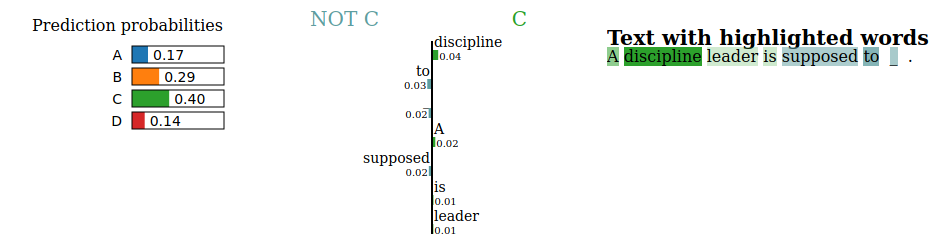
\includegraphics[scale=0.35]{images/lime-result-q-1a}
	\caption{\emph{LIME} result for the first experiment with original example.}
	\label{fig:lime-result-q-1a}
\end{figure}
\paragraph{}
In that example, the real label was $C$, and \emph{LIME} was able to detect that the important word was ``discipline'', so if we change this word the result will vary, but if we change the rest of the question, the result shouldn't change too much. 
So the next steps were to check if that idea was true. In order to do this some changes have been made in both the question and the options to see if the result is the same.
\paragraph{}

\section{Model-specific experiments}
\label{sec:ModelSpecificExperiments}
\noindent 
\subsection{Attention Heatmap}
\label{sec:AttentionHeatmapResults}
\noindent As said before, to visualize the \emph{Attention} values as a heatmap is a common method (first introduced in the original \emph{Attention} paper, \cite{Bahdanau2014}. 
\paragraph{}
To visualize the \emph{Attention} heatmap is an easy way to see how tokens relate with each others, which may help to understand what is going on inside the model. Although after several experiments (not only of this method but others, as wil be seen after) it has been seen that the \emph{Attention} values is not really useful to explain why the model has predict an specific output instead of another one, it can be used, as seen, to detect patterns, useless heads and so on.
\paragraph{}
As an explainability method it is true that it is not as helpful as other methods that are indeed trying to explain the model output. But it can be used to detect if the model is underfitted (or overfitted), which may explain a wrong prediction. But it does not help to explain a right prediction.
\paragraph{}
In this case a simple heatmap has been plotted to see how \emph{tokens} at the question attend to \emph{tokens} at each of the options. As the \emph{attention} heatmap takes the \emph{attention} values of each of the heads, it has been decided to make the sum of the values of each head to get a unique value of each \emph{token} relationship. This way, the heatmaps of figures \ref{fig:attention-heatmap-c} and \ref{fig:attention-heatmap-examples} shows the sum of the \emph{attention} values of each head of \emph{tokens} in x-axis attending to \emph{tokens} in y-axis.
\paragraph{}
As can be seen in Fig \ref{fig:attention-heatmap-c}, the \emph{discipline token} that is the most important one (according to other methods and having into account that is the \emph{token} that differs with other types of leaders in the text) has not a special value or relationships with other important \emph{tokens} in the sentence, such as \emph{nobody chats in class}. 
\begin{figure}[h]
	\centering
	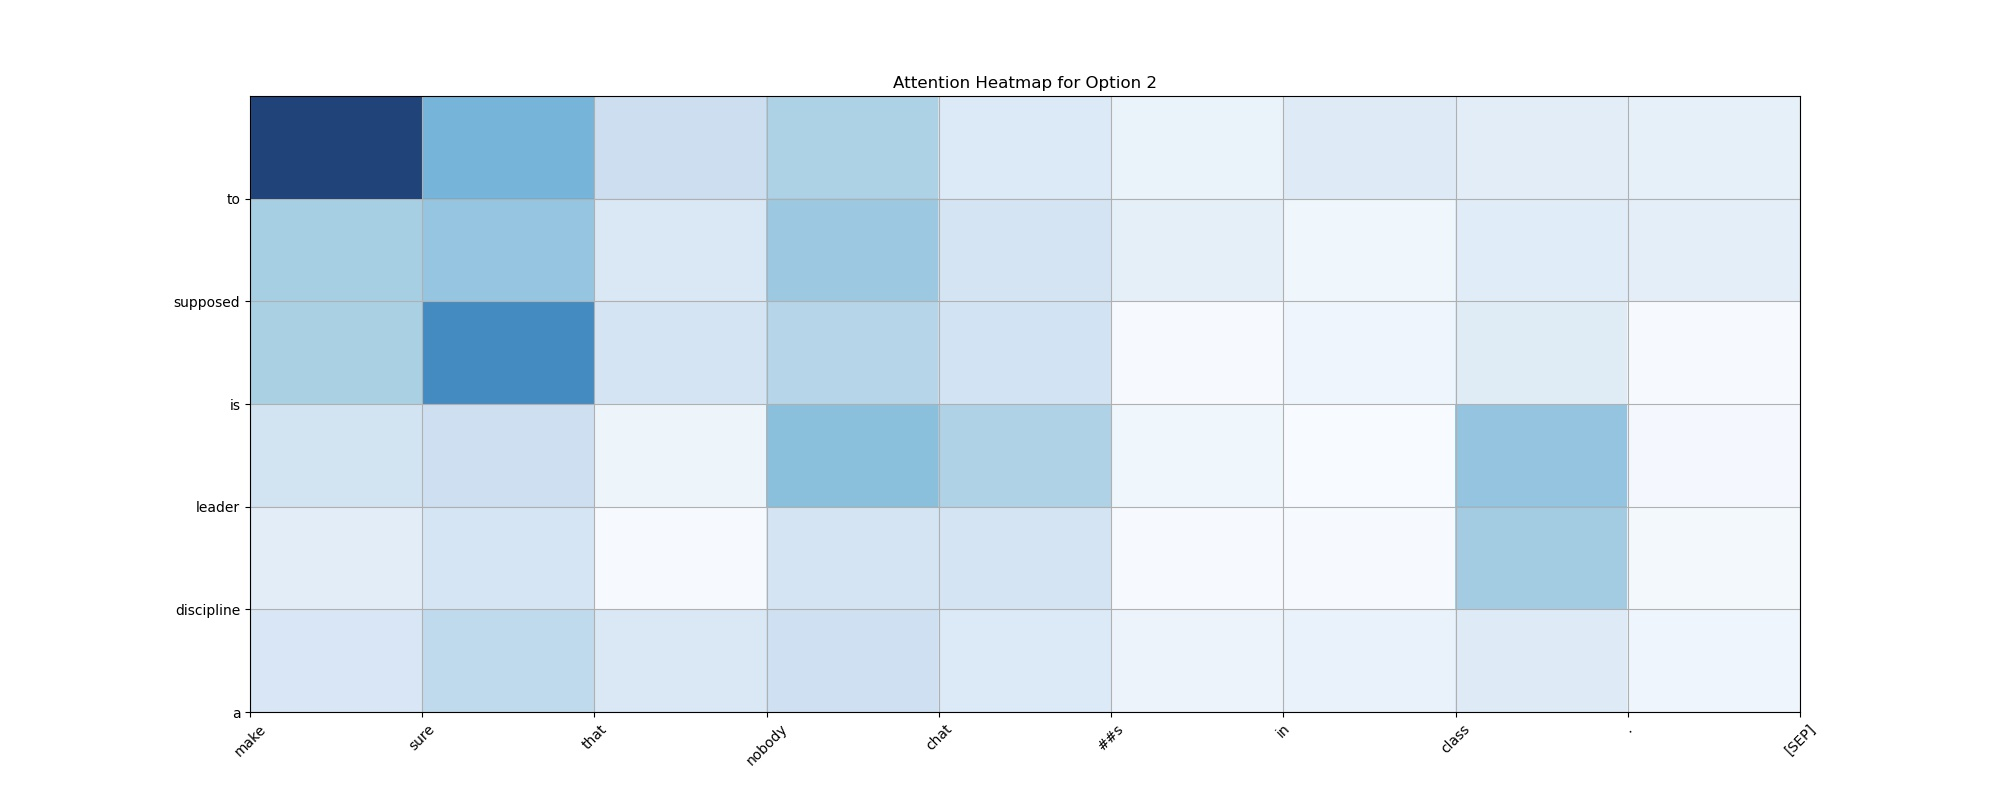
\includegraphics[scale=0.35]{images/attention_heatmap_2}
	\caption{\emph{Attention} heatmap for correct answer.}
	\label{fig:attention-heatmap-c}
\end{figure}
\paragraph{}
However, when looking at the heatmaps of other options, Fig \ref{fig:attention-heatmap-examples}, it can be seen that the \emph{discipline token} has higer values when attending to \emph{homework}, something that can have learnt during the training, as someone with discipline is someone that always does the homework. Also when looking at the whole picture (heatmap of each option), it can be seen that there is no a special pattern or something that helps to understand the model decision. 
\begin{figure}[h]
\centering
\begin{subfigure}{0.45\textwidth}
  \centering
	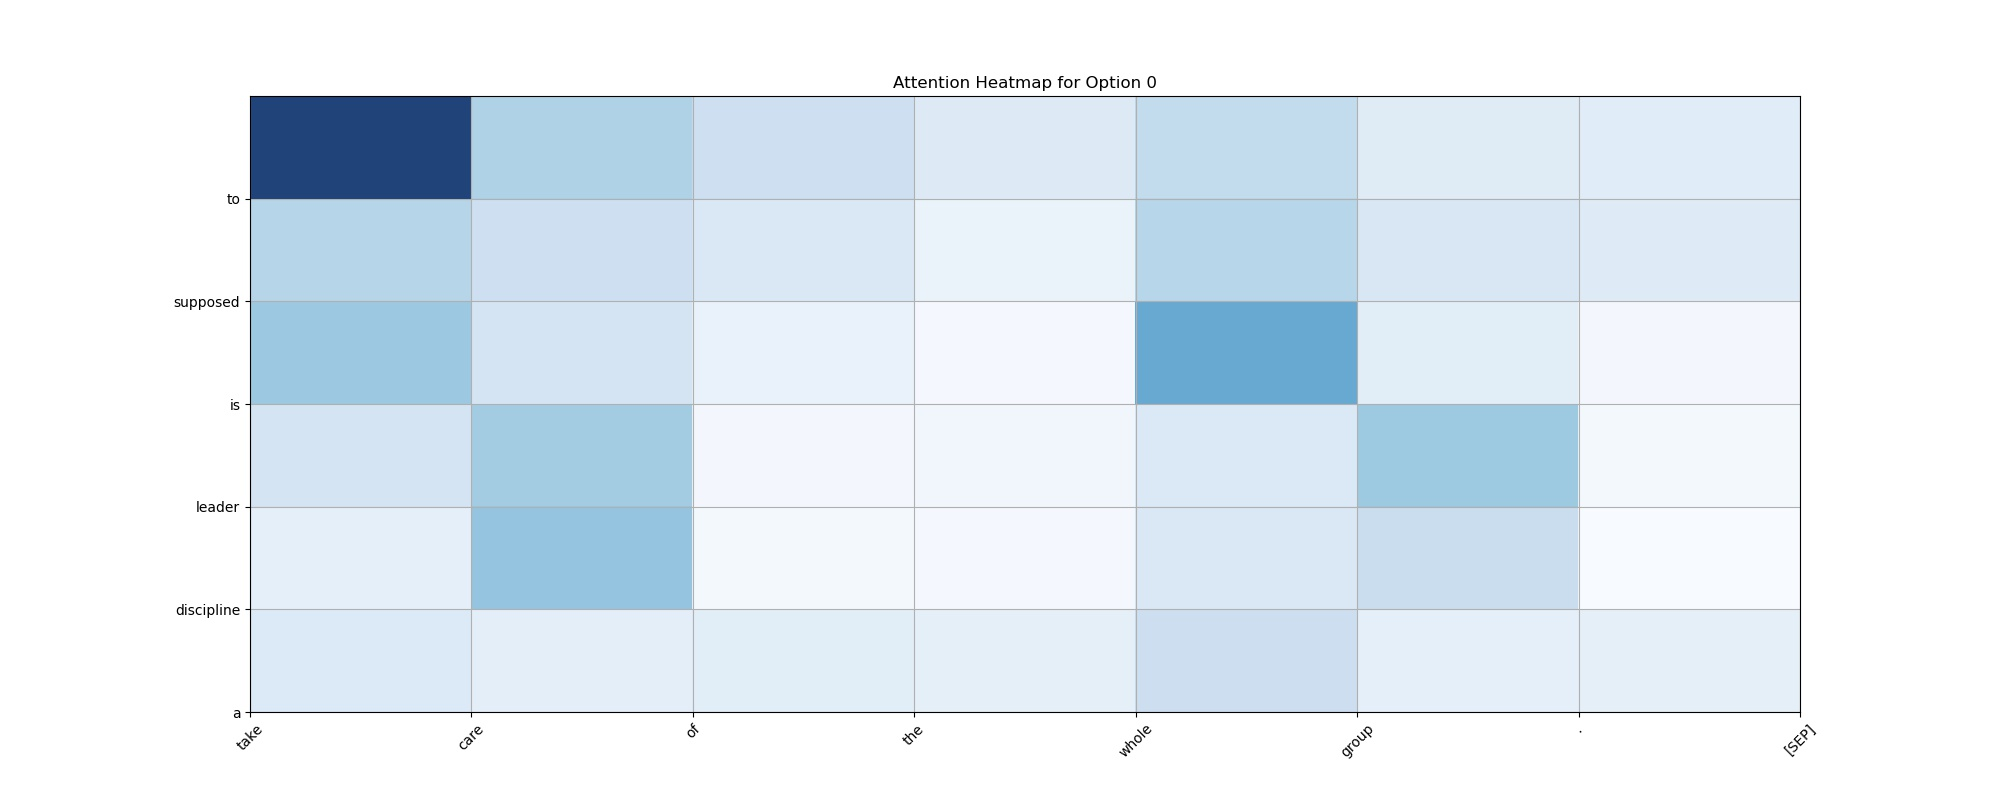
\includegraphics[width=200px]{images/attention_heatmap_0}
	\caption{\emph{Attention} heatmap option A.}
	\label{fig:att-hm-a}
\end{subfigure}
% \medskip\\
\begin{subfigure}{0.45\textwidth}
  \centering
	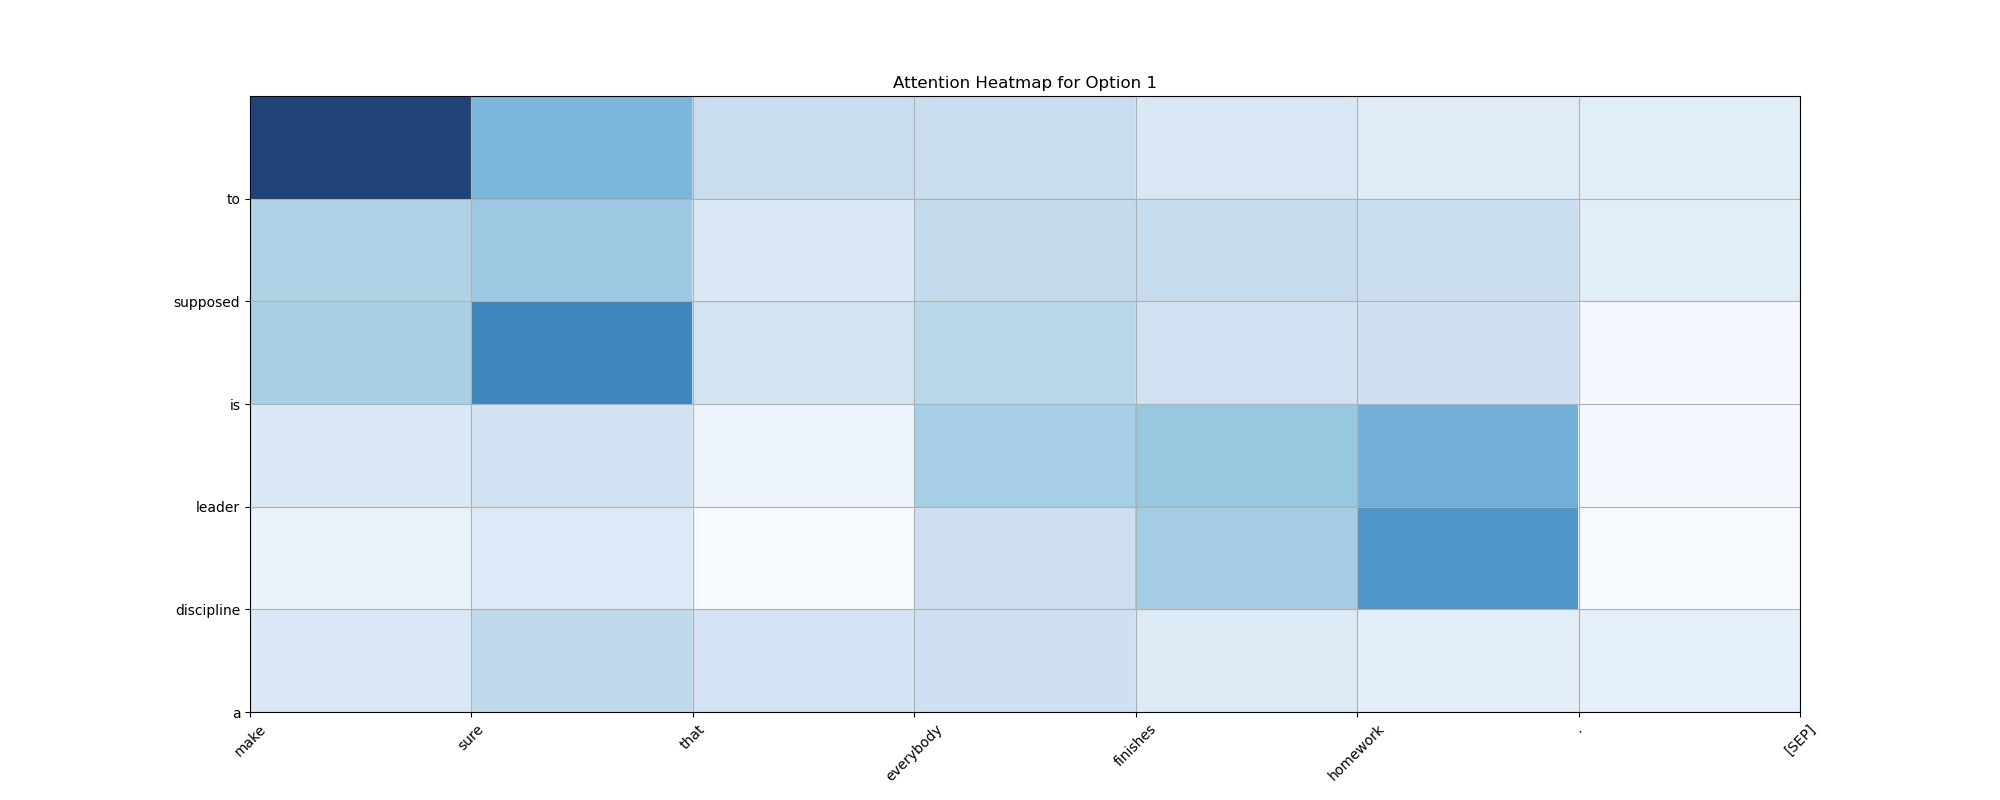
\includegraphics[width=200px]{images/attention_heatmap_1}
	\caption{\emph{Attention} heatmap option B.}
	\label{fig:att-hm-b}
\end{subfigure}
\medskip\\
\begin{subfigure}{0.45\textwidth}
  \centering
	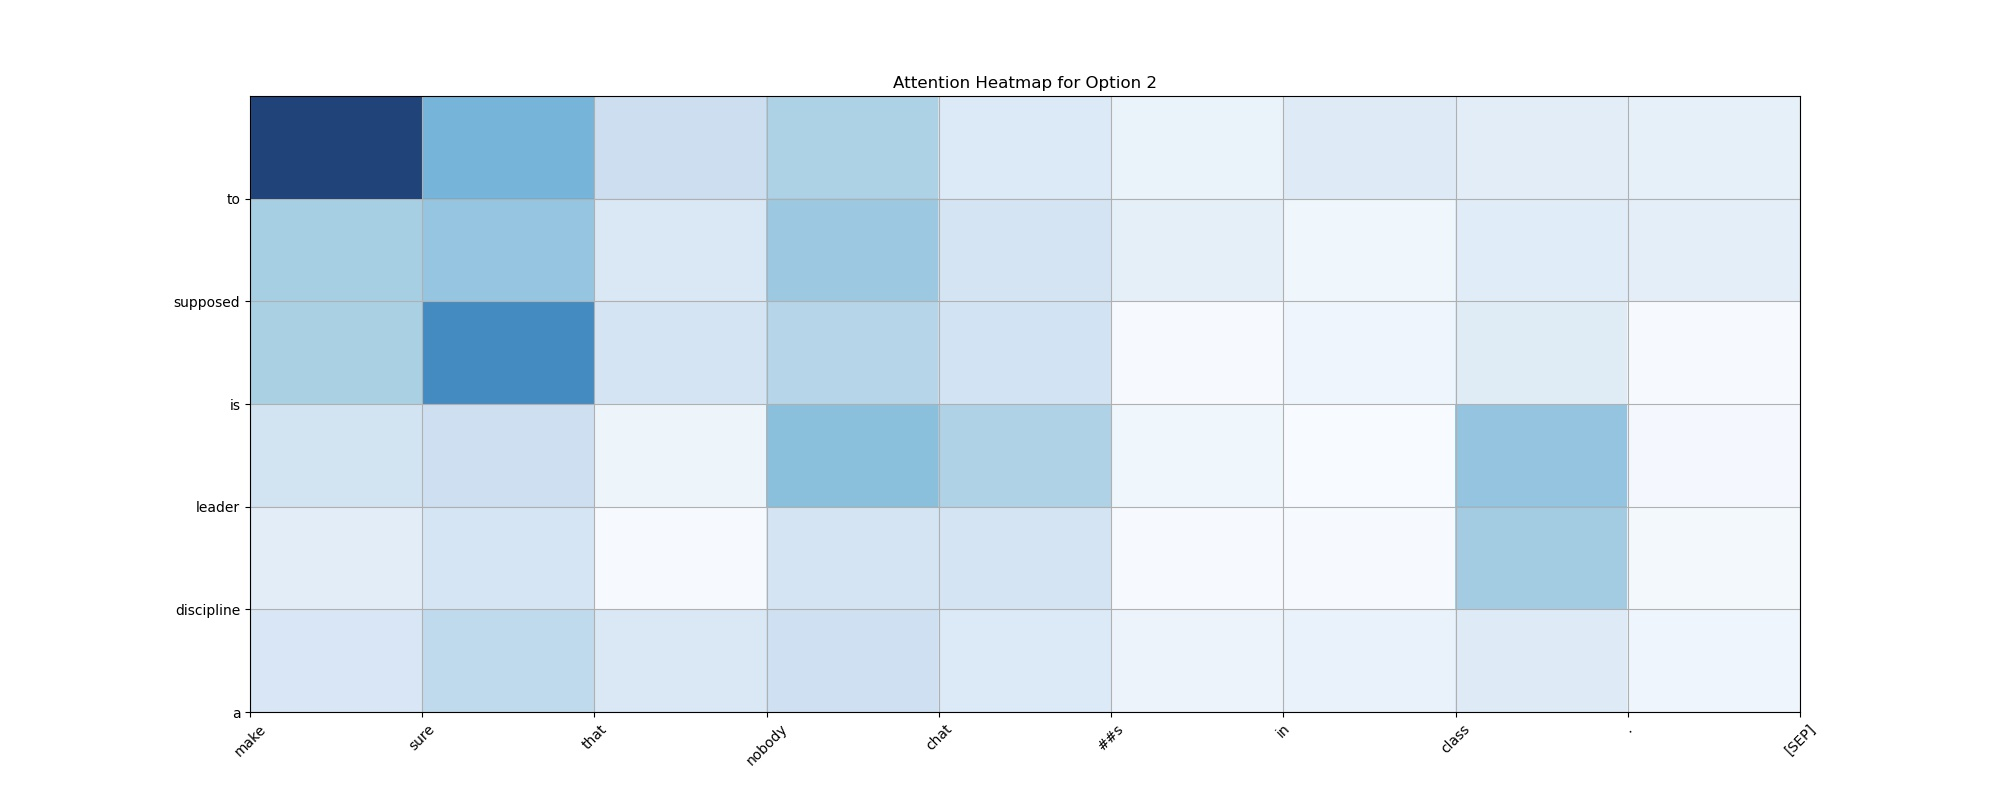
\includegraphics[width=200px]{images/attention_heatmap_2}
	\caption{\emph{Attention} heatmap option C.}
	\label{fig:att-hm-c}
\end{subfigure}
% \medskip\\
\begin{subfigure}{0.45\textwidth}
  \centering
	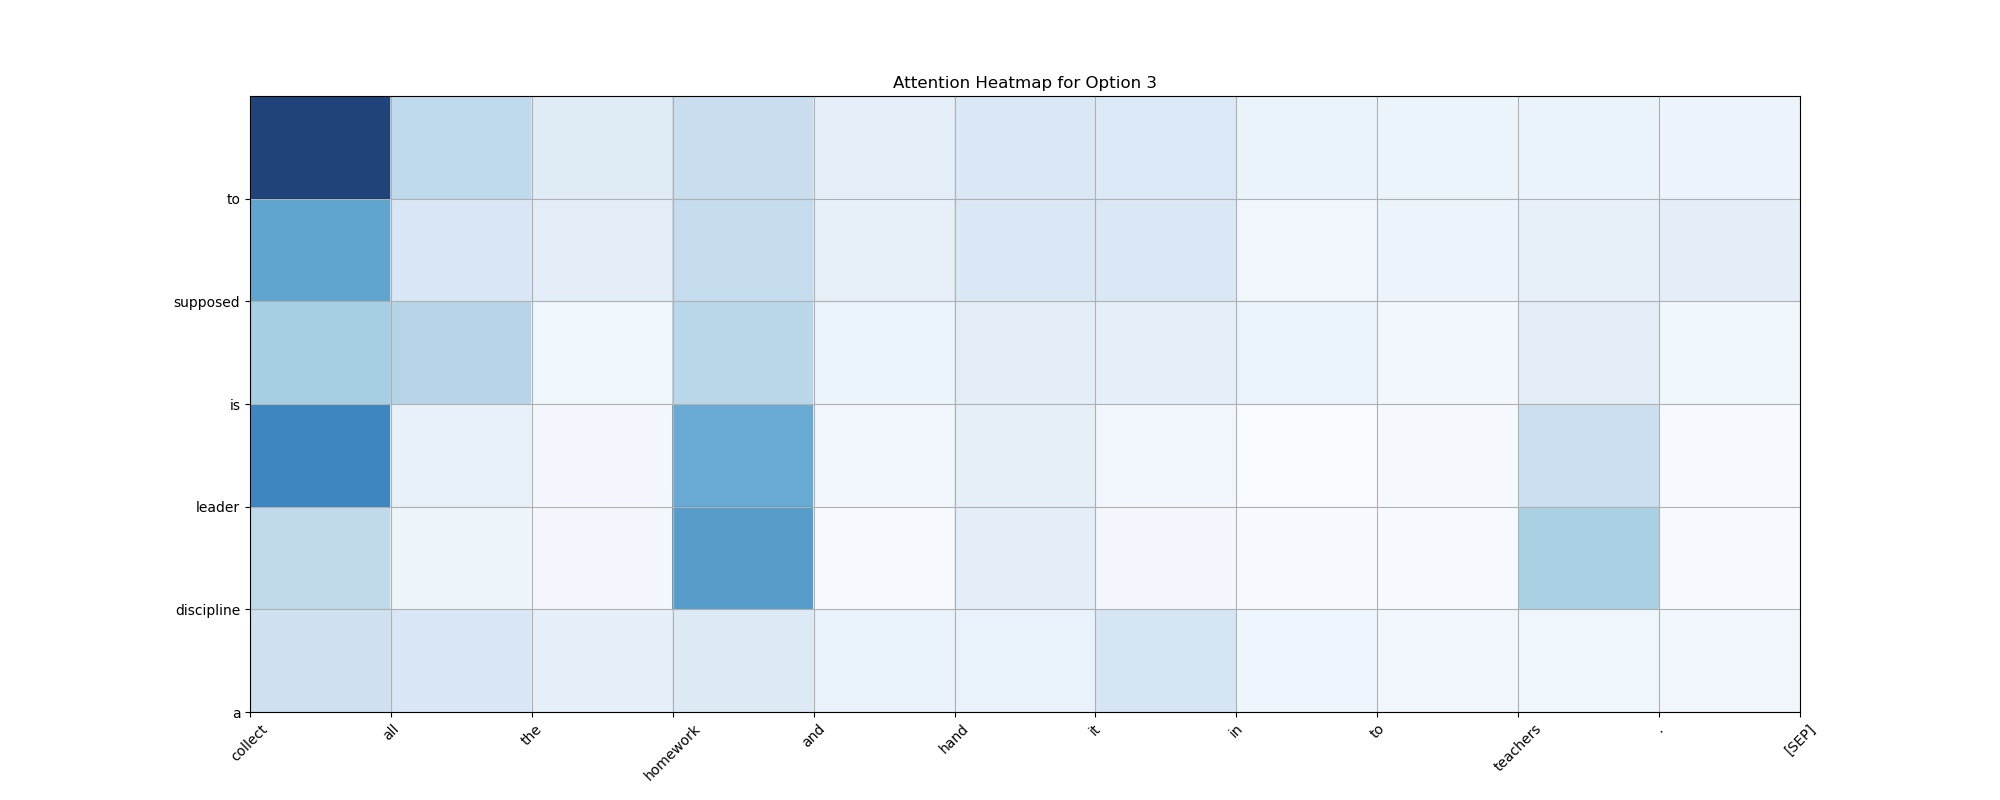
\includegraphics[width=200px]{images/attention_heatmap_3}
	\caption{\emph{Attention} heatmap option D.}
	\label{fig:att-hm-d}
\end{subfigure}
\caption{\emph{Attention} Heatmaps.}
\label{fig:attention-heatmap-examples}
\end{figure}


\subsection{BertViz}
\label{sec:BertVizResults}
\noindent Due to the problems of \emph{BertViz} to deal with large inputs, only has been tested the relations regarding the question and a single answer. This is, however, enough to test the tool, because it works in the same way no matter the input and, as it does not have to process anything, it does not matter the input used to test the tool and see how it works and how much information provides.
\paragraph{}
The first and most common way to study the \emph{Attention} layers is to use the \emph{Head View}, in which \emph{BertViz} shows the \emph{Attention} weights of a single layer. Again, the example used to test the tool has been: \textit{A discipline leader is supposed to  \_  .} 
\paragraph{}
When looking at how \emph{tokens} in Question attend to \emph{tokens} in each Answer, it can be seen that there is not anything that clarifies why the model chooses an option among the other. Figure \ref{fig:bertviz-q-options} shows layer 0 for each option. It can be seen that, for instance, \emph{discipline} attends more to \emph{tokens} such as \emph{class} or \emph{homework}, what makes sense. 
\begin{figure}[h]
\centering
\begin{subfigure}{0.4\textwidth}
  \centering
	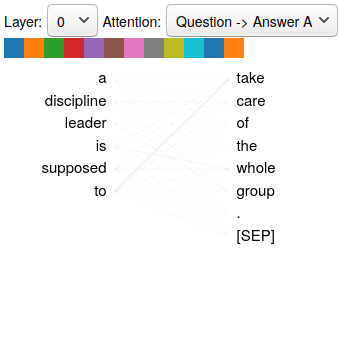
\includegraphics[width=120px]{images/bertviz-question-a}
	\caption{Question attending to Answer A.}
	\label{fig:bertviz-q-aa}
\end{subfigure}
\medskip
\begin{subfigure}{0.4\textwidth}
  \centering
	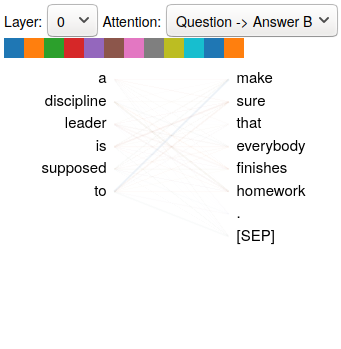
\includegraphics[width=120px]{images/bertviz-question-b}
	\caption{Question attending to Answer B.}
	\label{fig:bertviz-q-ab}
\end{subfigure}
\medskip\\
\begin{subfigure}{0.4\textwidth}
  \centering
	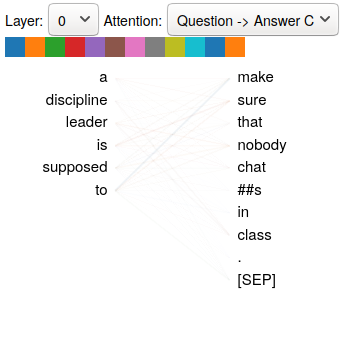
\includegraphics[width=120px]{images/bertviz-question-c}
	\caption{Question attending to Answer C.}
	\label{fig:bertviz-q-ac}
\end{subfigure}
\medskip
\begin{subfigure}{0.4\textwidth}
  \centering
	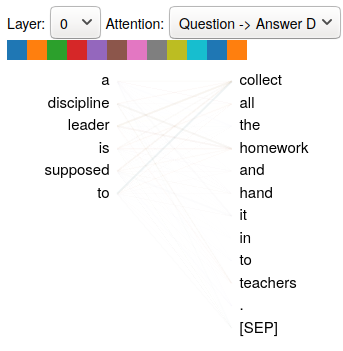
\includegraphics[width=120px]{images/bertviz-question-d}
	\caption{Question attending to Answer D.}
	\label{fig:bertviz-q-ad}
\end{subfigure}
\caption{\emph{BertViz} Head View of Question to Answers.}
\label{fig:bertviz-q-options}
\end{figure}
\paragraph{}
For instance, it can be seen in Figure \ref{fig:bertviz-l11h2} that \emph{discipline} attends to \emph{make sure that nobody}, which is really related to \emph{discipline}. However, there are different patterns across the layers and heads, and each head in each layer attend to \emph{tokens} by following a specific pattern. 
\begin{figure}[!h]
	\centering
	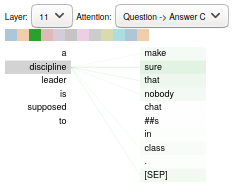
\includegraphics[scale=0.4]{images/bertviz-question-l11-head2}
	\caption{\emph{BertViz} layer 11, head 2.}
	\label{fig:bertviz-l11h2}
\end{figure}
\paragraph{}
As there are usually too many heads (model used has 12 heads per each one of the 12 layers), it costs a lot to look at each one separately. In order to take a global look and to discover patterns and useless heads, the \emph{BertViz Model View} is used. In Figure \ref{fig:bertviz-model-q} it can be seen that the \emph{Attention} layers follow patterns, even when the option change.
\begin{figure}[!h]
\centering
\begin{subfigure}{0.4\textwidth}
  \centering
	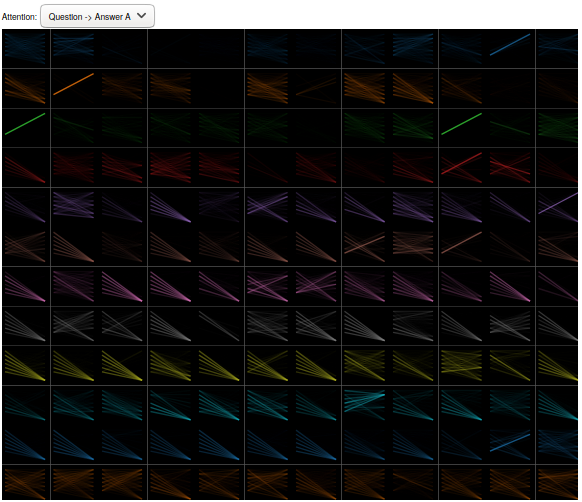
\includegraphics[width=140px]{images/bertviz-model-a}
	\caption{Question attending to Answer A.}
	\label{fig:bertviz-model-q-aa}
\end{subfigure}
\medskip 
\begin{subfigure}{0.4\textwidth}
  \centering
	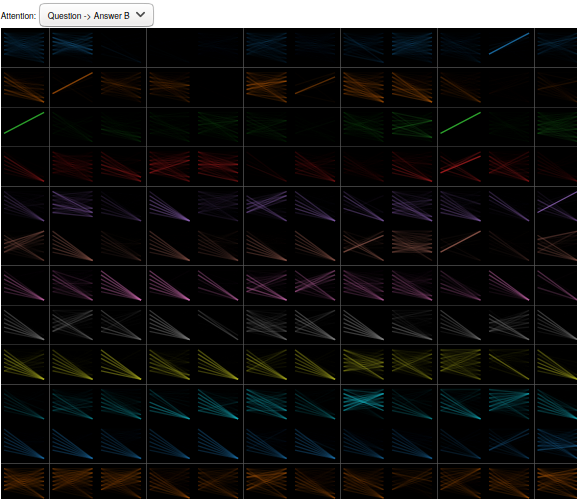
\includegraphics[width=140px]{images/bertviz-model-b}
	\caption{Question attending to Answer B.}
	\label{fig:bertviz-model-q-ab}
\end{subfigure}
\caption{\emph{BertViz} Model View of Question to Answers A and B.}
\label{fig:bertviz-model-q}
\end{figure}
\paragraph{}
Once that a pattern have been detected (or an outlier) it's useful to look at that specific head. The tool let the user to do this by clicking in the corresponding head, Figure \ref{fig:bertviz-model-head}. This way the user can see what \emph{tokens} are being attended at in the patterns, e.g. nouns, prepositions, etc. 
\begin{figure}[!h]
	\centering
	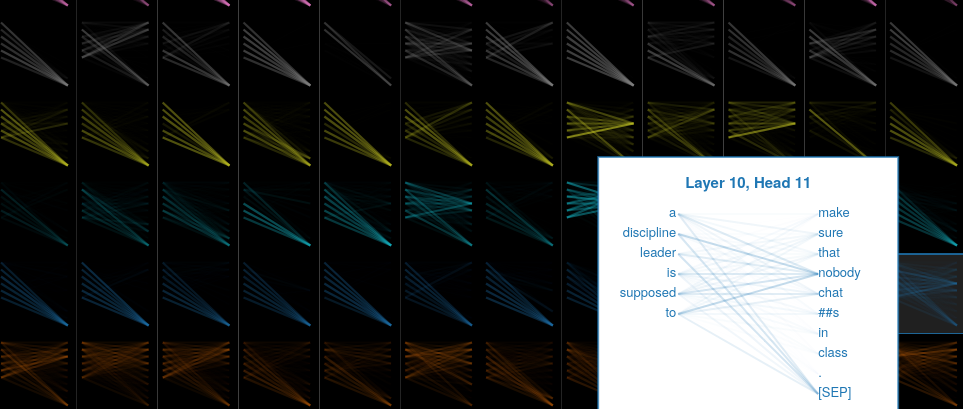
\includegraphics[scale=0.4]{images/bertviz-model-detail}
	\caption{To look at a single head in the Model View of \emph{BertViz}.}
	\label{fig:bertviz-model-head}
\end{figure}
\paragraph{}
The model view is useful to have a global look of the model, to see its behaviour and to see what heads are useful/useless. For instance, it can be seen that a lot of heads follow the same pattern, all \emph{tokens} attend to the \emph{[SEP] token}, what is considered as a \emph{null head}. These heads, therefore, could be prune to save space and time. This could be due to the training of the model, meaning that the model could be underfitted and, therefore, should be trained with more data or during more time, which in this case is true, because due to hardware and temporal limitations the model has been training for just 1 day, which is not enough for a \emph{LM}.
\paragraph{}
Therefore, to look at the \emph{Attention} does not really provide an explanation of why the model choose one option, because it follows patterns and does not change over the different options. 
\paragraph{}
Although \emph{BertViz} does not help to explain a prediction of the model, it is a good tool for visualizing the \emph{Attention} weights, what can be useful as said before to, for instance, prune useless heads. But it's not a good option for explain a prediction of the model.

\cleardoublepage
\subsection{Intrinsic GPT-3}
\label{sec:GPT3Results}
\noindent To force \emph{GPT-3} to generate the explanations (or any expected result), first a few examples of what exactly is desired have to be feed to the model in order to show it what is expected.
\paragraph{}
In this case, three passages were selected from the test set to feed \emph{GPT-3} and force it to generate the text as wished, this is, an explanation of the answer. These passages were complex to answer, beacuse in some of them the answer was not in the text itself, but related to. For instance, in one of the passages the question asks about the location of the story, given as options: England; America; Japan; Australia. But in the text it talks about New York, so a bit of commonsense is needed in order to relate New York with America.
\paragraph{}
The examples feed to the model included the context, the question, the options, the correct answer and a simple explanation of why it is the correct answer. The appendix \ref{ch:GPT3-Examples} includes all the examples feed to the model. 
\paragraph{Example 1}
The first try was using the Example 1, \ref{ex:1}. As the answer was in the text it was not surprising that \emph{GPT-3} predicted it correctly. Regarding the explanation, Figure \ref{fig:gpt3-ex1}, it is a good explanation but, again, as the answer is inside the text there was not too much to explain but say that the article says so.
\begin{figure}[h]
	\centering
	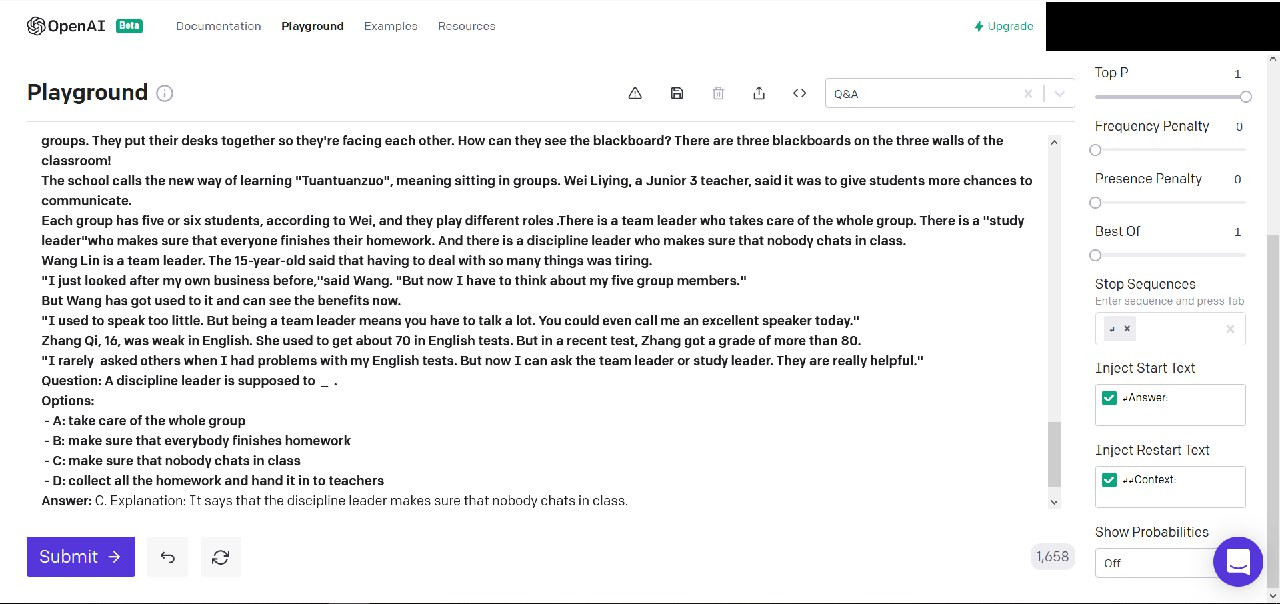
\includegraphics[scale=0.25]{images/gpt3-ex1}
	\caption{Explanation of GPT3 for the Example 1.}
	\label{fig:gpt3-ex1}
\end{figure}
\paragraph{Example 2}

\paragraph{}
Surprisngly, the result of \emph{GPT-3} included the correct answer and an accurately explanation, \ref{fig:gpt3-result-correct}.
\begin{figure}[h]
	\centering
	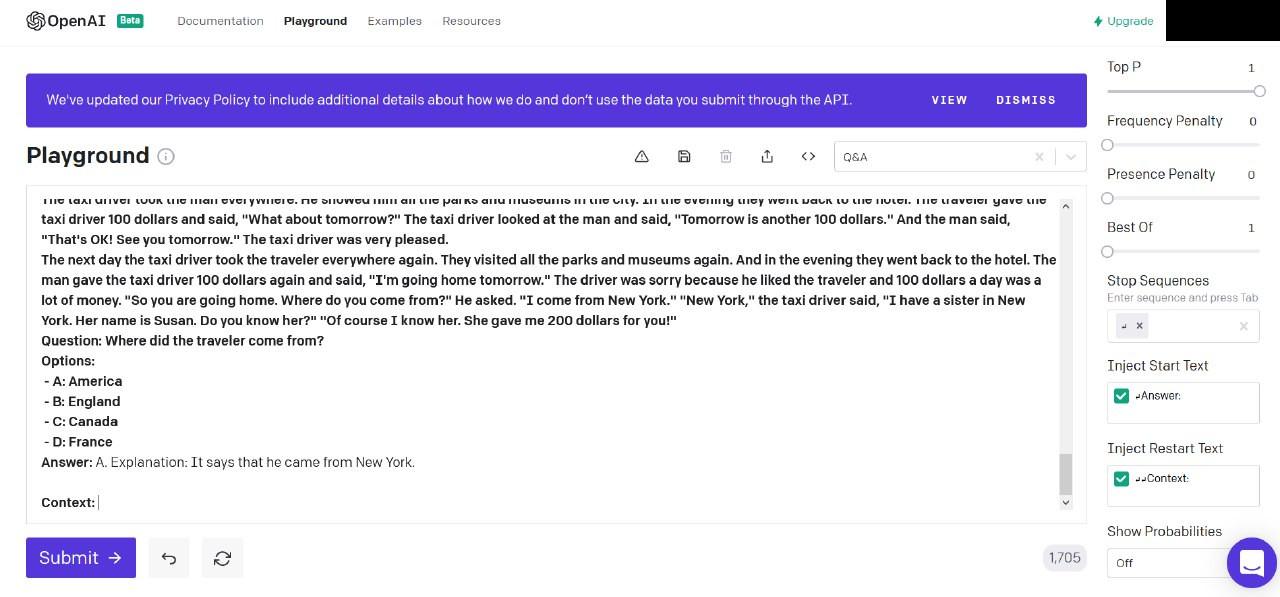
\includegraphics[scale=0.25]{images/gpt3-correct}
	\caption{Explanation of GPT3.}
	\label{fig:gpt3-result-correct}
\end{figure}
\paragraph{}
But it has been detected that it is not always that good, and therefore it is not clear if it's indeed able to explain itself. With a simple change of options, interchanging the options A and B, the result fails in the prediction, the explanation is the same though, \ref{fig:gpt3-result-fail1}. And if an extra ``answer'' token is added to the end, the result of the prediction is correct but it fails in the explanation, \ref{fig:gpt3-result-fail2}.
\begin{figure}[h]
	\centering
	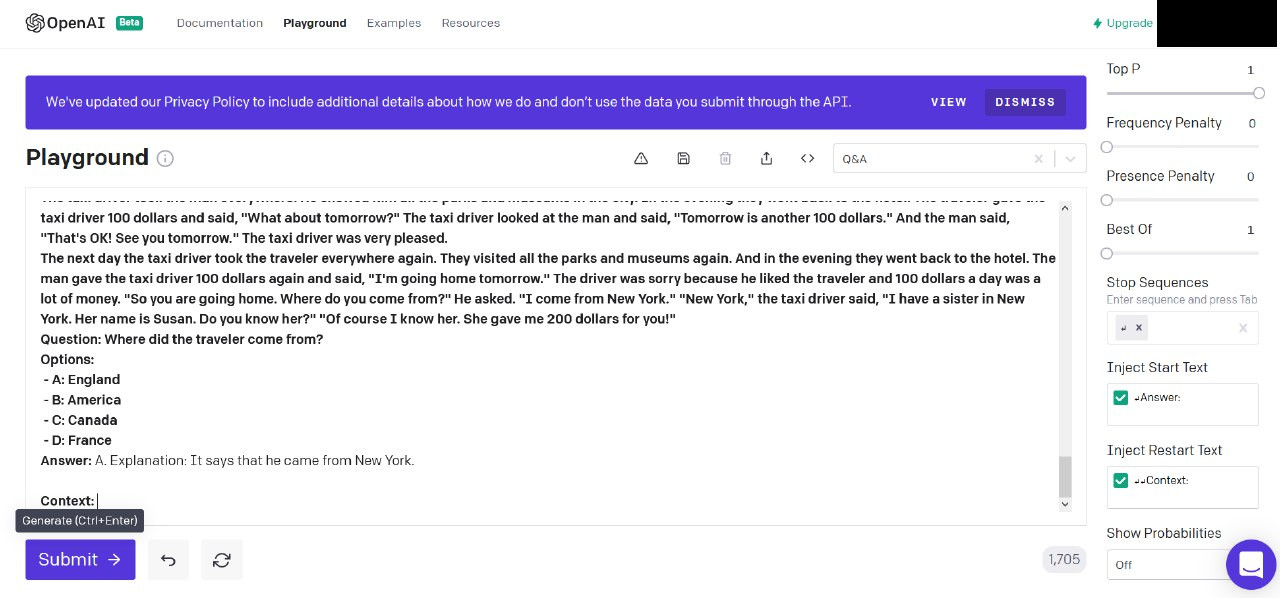
\includegraphics[scale=0.25]{images/gpt3-fail1}
	\caption{Wrong prediction of GPT3.}
	\label{fig:gpt3-result-fail1}
\end{figure}
\begin{figure}[h]
	\centering
	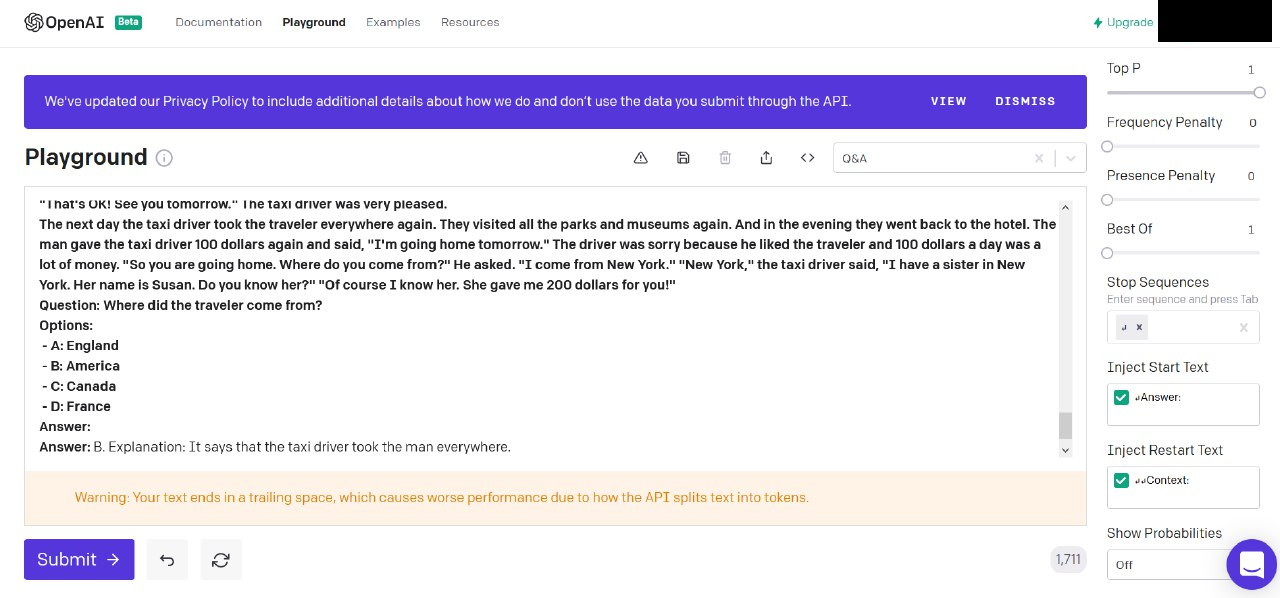
\includegraphics[scale=0.25]{images/gpt3-fail2}
	\caption{Wrong explanation of GPT3.}
	\label{fig:gpt3-result-fail2}
\end{figure}
%%%%%%%%%%%%%%%%%%%%%%%%%%%%%%%%%%%%%%%%%%%%%%%%%%%
%%% CONCLUSIONES Y TRABAJO FUTURO
%%%%%%%%%%%%%%%%%%%%%%%%%%%%%%%%%%%%%%%%%%%%%%%%%%%

\chapter{Conclusions and Future Work}
\fancyhead[RE]{\textsc{Chapter} \thechapter. Conclusions and Future Work}
\label{ch:ConclusionsAndFutureWork}
\section{Conclusions}
\label{sec:Conclusions}
\noindent To explain \emph{black box} models such as deep learning models it is a really complex task that, despite of the efforts of the researchers, is still a challenge far away from being completely solved. 
\paragraph{}
Among the last years researchers have developed some interesting approaches that are really helpful to understand the model behavior and to know a bit more about why the model has given an output instead of another one. These approaches are based on some different techniques that help the user to understand what is going on inside the model when giving an output, and to make it easier for the user are often presented with visualization tools and techniques that make really simple to understand the explanations. 
\paragraph{LIME} After several experiments, it can be seen that \emph{LIME} is able to detect the most important words (or spans) the model focus on when making its prediction. But it's still not clear why the model makes a prediction, because \emph{LIME} explains the most important words for each class, but does not explain why the model choose a class over the other ones.
\paragraph{}
This way, \emph{LIME} can help to understand the words that are important for the prediction, an this can help to understand the best way to create questions or to give the model the correct options. But it have been also seen that to change this words or this options does not mean the model is going to change its prediction. For instance, in the experiments in which the most important word ``discipline'' was replaced with a synonym ``orderliness'', the model predicted the good label meanwhile with the word ``discipline'' that appeared in the original text the model did not, and in the experiment in which the options given to the model were perturbed trying to preserve all the important words in the original question (like ``supposed'') the model also failed in its prediction.
\paragraph{}
So it is not clear which one is the correct way to make a question, or why the model has chosen a class instead of another one.
Besides this, when the model fails, \emph{LIME} does not really help to know why the model has failed, because the explanations of each of the classes will give us the important words for that class, but will not tell why a class is chosen beyond the others. 
\begin{figure}[!h]
	\centering
	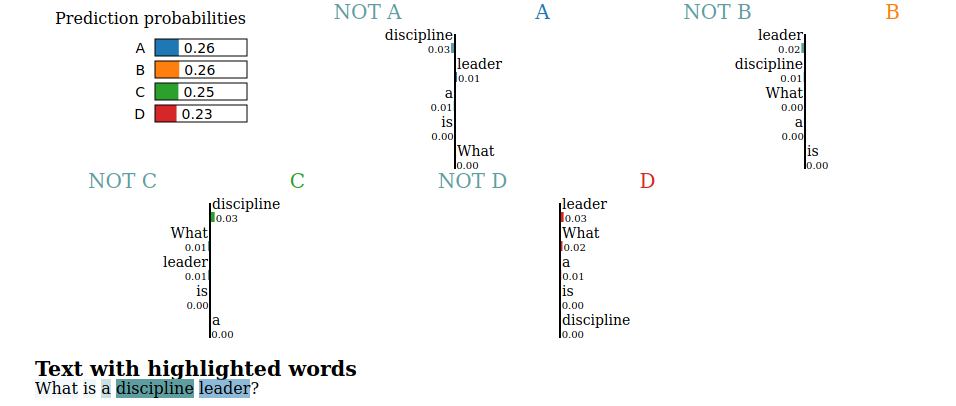
\includegraphics[scale=0.35]{images/conclussionLime}
	\caption{Explanation of all options given by \emph{LIME}}
	\label{fig:conclussionLime}
\end{figure}
\paragraph{BertVIZ} \emph{BertViz} is a tool to explore and visualize \emph{attention} weights in every \emph{transformer-based} model. It allows the user to visualize \emph{attention} weights in an easy and user-friendly way, making possible to see and detect bias and patterns in the \emph{attention} mechanism as well as to detect useless heads to be able to prune them and save space and time without loosing performance.
\paragraph{}
But, \emph{BertViz} is just that, a visualization tool. It does not provide or perform any additional operation over the model and, therefore, it does not help more than other visualization tools to understand what is going on inside the model. Although, as said before, it helps to visualize \emph{attention} weights to, for instance, detect patterns or see how words relate with others, this is not helpful when trying to understang the model behaviour and to know why the model has given an output and why not another one. But \emph{BertViz} is not guilty for this, because as some research articles\cite{} has pointed out recently, to visualize the \emph{attention} weights does not really provide an explanation of the local prediction, because the \emph{attention} mechanism is just used to generate contextual embeddings of the input. Instead of that it would be more useful to explain the final layers of the model, that are the ones that are really solving the task, but this is very difficult, as they have as input the embeddings generated by the full model, making it really difficult to explain the layers behavior and to understand the explanations.
\paragraph{}
Therefore, other techniques such as \emph{LIME} that create a surrogate explainable model are more useful than to visualize the \emph{attention} weights in order to explain the model behavior.
\paragraph{GPT-3}
Despite of having some good explanations from \emph{GPT-3} explaining itself, it is not clear if \emph{GPT-3} is able to explain itself. When the explanation is in the article or it's easy to explain, it has not problem to do it. But when the question or the explanation are more difficult, not always give a valid explanation (sometimes nor even a good answer).
\paragraph{}
Although the explanations are not always valid, they are gramatically correct, taking sentences from the article. But sometimes they are not even related to the question, other times it gives the correct explanation, as in \ref{fig:gpt3-result-correct}, where the option was \emph{America} and the explanation is: \emph{It says that he came from New York}, which is indeed in America but the lack of explanation relating New York to America could make it a bad explanation that is not enough for a user to understand the result, as seen in \ref{sec:qa-evaluation}, the completeness was one of the \emph{criteria} used by \cite{Allam2012} to select an answer as correct. Did the model relate New York with America to choose it as the result and the explanation? or did it just focus on that the question was asking for a place? This is not clear as the explanation was not consistent and not complete. So, this explanation, as seen in \ref{sec:qa-evaluation} and following the classification of \cite{Pablo-Sanchez}, this answer could be classified as incomplete. But this classification was thought for answers of \emph{QA} systems, not for explanations. As seen in \ref{sec:xai-evaluation} there is not a common way to evaluate the explanations what can lead to a lack of quality in the results. For instance in this case, in which \emph{GPT-3} is giving an explanation in natural language, it is easier to understand for the user, but the explanation is not consistent nor complete, so the answers classification could be used for this type of explanations.
\section{FutureWork}
\label{sec:FutureWork} 

%%%%%%%%%%%%%%%%%%%%%%%%%%%%%%%%%%%%%%%%%%%%%%%%%%%
%%% BIBLIOGRAF�A
%%%%%%%%%%%%%%%%%%%%%%%%%%%%%%%%%%%%%%%%%%%%%%%%%%%
\bibliographystyle{fullname_esp}
\cleardoublepage
\addcontentsline{toc}{chapter}{References}
\chapter*{References}
\fancyhead[RE]{References}
\fancyhead[LO]{References}

\nocite{*}
\bibliography{bibliography}

\newpage
\newpage

%%%%%%%%%%%%%%%%%%%%%%%%%%%%%%%%%%%%%%%%%%%%%%%%%%%
%%% APENDICES SI PROCEDE (COMENTAR)
%%%%%%%%%%%%%%%%%%%%%%%%%%%%%%%%%%%%%%%%%%%%%%%%%%%
\appendix
\fancyhead[RE]{\textsc{APPENDIX} \thechapter. GPT-3 Examples}
\fancyhead[LO]{\textsc{APPENDIX} \thechapter. GPT-3 Examples}
%%%%%%%%%%%%%%%%%%%%%%%%%%%%%%%%%%%%%%%%%%%%%%%%%%%
%%% CONCLUSIONES Y TRABAJO FUTURO
%%%%%%%%%%%%%%%%%%%%%%%%%%%%%%%%%%%%%%%%%%%%%%%%%%%

\chapter{Examples feed to GPT-3}
\label{ch:GPT3-Examples}
\noindent As said before, to force \emph{GPT-3} to output an expected result, it has to be feed with some examples of the desired output to know what has to generate. In order to force it to generate explanations of the prediction, first a few examples of the test set has been formatted and added an explanation as desired. These are the full examples feed to \emph{GPT-3}:

\begin{passage}[Article of GPT Example 1]{art:gpt1}
 It was the golden season. I could see the yellow leaves dancing in the cool wind. I felt lonely and life is uninteresting. But one day, the sound of a violin came into my ears. I was so surprised that I ran out to see where it was from. A young girl, standing in the wind, was lost in playing her violin. \\
I had never seen her before. The music was so wonderful that I forgot who I was. \\
Leaves were still falling. Every day she played the violin in the same place and I was the only listener. It seemed that I no longer felt lonely and life became interesting. We didn't know each other, but I thought we were already good friends.
One day, when I was listening, the sound suddenly stopped. The girl came over to me. \\
``You must like violin.'' she said. \\
``Yes. And you play very well. Why did you stop?'' I asked. \\
Suddenly, a sad expression appeared on her face and I could feel something unusual. \\
``I came here to see my grandmother, but now I must leave. I once played very badly. It is your listening every day that has \_ me.'' she said. \\
``In fact, it is your music that has given me those meaningful days.'' I answered. ``Let us be friends.'' \\
The girl smiled and I smiled. \\
I never heard her play again in my life. Only thick leaves were left behind. But I will always remember the girl. She is like a dream; so short, so bright that it makes life beautiful. \\
There are many kinds of friends. Some are always with you, but don't understand you. Some say only a few words to you, but are close to you. I shall always think of those golden days and the girl with the violin. She will always bring back the friendship between us. I know she will always be my best friend.
\end{passage}
Q: ``\emph{What's the best title for the passage?}''\\
Options: 
\begin{itemize}
 \item A: A Musical Girl
 \item B: Wonderful Music
 \item C: A Special Friend in a Special Autumn
 \item D: How to Be Friends
\end{itemize}
Answer: C. \\
Explanation: It says that it was the golden season and autumn is known as the golden season and it speaks about friendship not just music.

\begin{passage}[Article of GPT Example 2]{art:gpt2}
 Is it important to have breakfast every day? A short time ago, a test was given in the United States. People of different ages, from 12 to 83, were asked to have a test. During the test, these people were given all kinds of breakfast, and sometimes they got no breakfast at all. Scientists wanted to see how well their bodies worked after eating different kinds of breakfast. \\
The results show that if a person eats a right breakfast, he or she will work better than if he or she has no breakfast. If a student has fruit, eggs, bread and milk before going to school, he or she will learn more quickly and listen more carefully in class. Some people think it will help you lose weight if you have no breakfast. But the result is opposite to what they think. This is because people become so hungry at noon that they eat too much for lunch. They will gain weight instead of losing it.
\end{passage}
Q: ``\emph{According to the passage, what will happen to you if you don't have any breakfast?}''\\
Options: 
\begin{itemize}
 \item A: To be healthier.
 \item B: To work better.
 \item C: To gain weight.
 \item D: To fail the test.
\end{itemize}
Answer: C. \\
Explanation: Because it says that people become so hungry at noon that they eat too much for lunch.

\begin{passage}[Article of GPT Example 3]{art:gpt3}
 It's the second time for me to come to Beijing. There are many places of interest in Beijing, such as the Summer Palace, the Great Wall, etc. What's more, I think great changes have taken place in Beijing. People's living conditions have improved a lot. Their life is very happy. Almost everyone has a big smile on the face. People in Beijing are in high spirits and hard-working. Children can receive a good education. \\
But in the past, some children didn't have enough money to go to school. They often worked for cruel bosses. The bosses didn't give them enough food. I feel sorry for them. Today people have already lived in tall building, worn beautiful clothes and so on. Life has changed greatly.
\end{passage}
Q: ``\emph{How many times has the writer been to Beijing?}''\\
Options: 
\begin{itemize}
 \item A: Once.
 \item B: Twice.
 \item C: Three time.
 \item D: Four times.
\end{itemize}
Answer: B. \\
Explanation: Because it says that is the second time that he goes to Beijing.

\begin{passage}[Article of GPT Example 4]{art:gpt4}
 Several years ago,a television reporter was talking to three of the most important people. One was a very rich banker,another owned one of the largest companies in the world,and the third owned many buildings in the center of New York. \\
The reporter was talking to them about being important. ``How do we know if someone is really important?'' the reporter asked the banker. \\
The banker thought for a few moments and then said, ``I think anybody who is invited to the White House to meet the President of the United States is really important.'' \\
The reporter then turned to the owner of the very large company. ``Do you agree with that?'' she asked. \\
The man shook his head, ``No. I think the President invites a lot of people to the White House. You'd only be important if while you were visiting the President, there was a telephone call from the president of another country,and the President of the US said he was too busy to answer it.'' \\
The reporter turned to the third man. ``Do you think so?'' \\
``No, I don't,'' he said. ``I don't think that makes the visitor important. That makes the President important. '' \\
``Then what would make the visitor important?'' the reporter and the other two men asked. \\
``Oh, I think if the visitor to the White House was talking to the President and the phone rang, and the President picked up the receiver, listened and then said, 'It's for you.' '' \\
\end{passage}
Q: ``\emph{This story happened in   \_  .}''\\
Options: 
\begin{itemize}
 \item A: England.
 \item B: America.
 \item C: Japan.
 \item D: Australia.
\end{itemize}
Answer: B. \\
Explanation: It talks about New York, the United states and the White House that are in America.

\begin{passage}[Article of GPT Example 5]{art:gpt5}
 Dear John, Thank you very much for your letter. I am glad that you enjoyed your holiday with me. We enjoyed having you and your sister here. We hope that you will both be able to come again next year. Perhaps you'll be able to stay longer next time you come. A week is not really long enough, is it? If your school has a five-week holiday next year, perhaps  you'll be able to stay with us for two or three weeks. \\
We have been back at school three weeks now. It feels like three months! I expect  that you are both working very hard now that you are in Grade One. I shall have to work hard next year when I am in Grade One. Tom and Ann won't be in Grade One until 2011.
They went for a picnic yesterday but I didn't go with them because I cut my foot and I couldn't walk very well. They went to an island and enjoyed themselves. Do you still remember the island? That's where all five of us spent the last day of our holiday.
Tom, Ann and I send our best wishes to Betty and you. We hope to see you soon. \\
Yours sincerely, \\
Michael
\end{passage}
Q: ``\emph{From the words of  ``It feels like three months!'' we know that  \_  .}''\\
Options: 
\begin{itemize} 
 \item A: Michael's teacher is very strict with the students.
 \item B: Michael is pleased with his school report.
 \item C: Michael has no interest in learning.
 \item D: Michael works very hard at his studies.
\end{itemize}
Answer: C. \\
Explanation: When something feels to go slower is because we don't like it. If we do like it seems to go faster.


% Publicaciones derivadas del trabajo realizado.


%%%%%%%%%%%%%%%%%%%%%%%%%%%%%%%%%%%%%%%%%%%%%%%%%%%
%%% lISTA DE TAREAS PENDIENTES.
%%%%%%%%%%%%%%%%%%%%%%%%%%%%%%%%%%%%%%%%%%%%%%%%%%%
\newpage
\newpage
%Eliminar si no hay todo's
\listoftodos


\end{document}

%%%%%%%%%%%%%%%%%%%%%%%%%%%%%%%%%%%%%%%%%%%%%%%%%%%
%%% SCRIPT FINAL DE TODO'S O TAREAS PENDIENTES.
%%%%%%%%%%%%%%%%%%%%%%%%%%%%%%%%%%%%%%%%%%%%%%%%%%%
% Make the margin par
\marginpar{%
    \begin{tikzpicture}[remember picture]%
        \draw node[notestyle] (inNote)
                 {#1};%
    \end{tikzpicture}%
}%
%
\begin{tikzpicture}[remember picture, overlay]%
    \draw[connectstyle]
        ([yshift=-0.2cm] inText)
            -| ([xshift=-0.2cm] inNote.west)
            -| (inNote.west);
\end{tikzpicture}%

}% 